\documentclass[a4paper]{article}
% generated by Docutils <http://docutils.sourceforge.net/>
\usepackage{fixltx2e} % LaTeX patches, \textsubscript
\usepackage{cmap} % fix search and cut-and-paste in Acrobat
\usepackage{ifthen}
\usepackage[T1]{fontenc}
\usepackage[utf8]{inputenc}
\usepackage{float} % float configuration
\floatplacement{figure}{H} % place figures here definitely
\usepackage{graphicx}
\setcounter{secnumdepth}{0}
\usepackage{longtable,ltcaption,array}
\setlength{\extrarowheight}{2pt}
\newlength{\DUtablewidth} % internal use in tables
\usepackage{tabularx}

%%% Custom LaTeX preamble
% PDF Standard Fonts
\usepackage{mathptmx} % Times
\usepackage[scaled=.90]{helvet}
\usepackage{courier}

%%% User specified packages and stylesheets

%%% Fallback definitions for Docutils-specific commands

% providelength (provide a length variable and set default, if it is new)
\providecommand*{\DUprovidelength}[2]{
  \ifthenelse{\isundefined{#1}}{\newlength{#1}\setlength{#1}{#2}}{}
}

% docinfo (width of docinfo table)
\DUprovidelength{\DUdocinfowidth}{0.9\textwidth}

% lineblock environment
\DUprovidelength{\DUlineblockindent}{2.5em}
\ifthenelse{\isundefined{\DUlineblock}}{
  \newenvironment{DUlineblock}[1]{%
    \list{}{\setlength{\partopsep}{\parskip}
            \addtolength{\partopsep}{\baselineskip}
            \setlength{\topsep}{0pt}
            \setlength{\itemsep}{0.15\baselineskip}
            \setlength{\parsep}{0pt}
            \setlength{\leftmargin}{#1}}
    \raggedright
  }
  {\endlist}
}{}

% titlereference role
\providecommand*{\DUroletitlereference}[1]{\textsl{#1}}

% hyperlinks:
\ifthenelse{\isundefined{\hypersetup}}{
  \usepackage[colorlinks=true,linkcolor=blue,urlcolor=blue]{hyperref}
  \urlstyle{same} % normal text font (alternatives: tt, rm, sf)
}{}
\hypersetup{
  pdftitle={HercuLeS 1.0 reference manual},
  pdfauthor={Nikolaos Kavvadias <nkavvadias@ajaxcompilers.com>}
}

%%% Title Data
\title{\phantomsection%
  HercuLeS 1.0 reference manual%
  \label{hercules-1-0-reference-manual}}
\author{}
\date{}

%%% Body
\begin{document}
\maketitle

% Docinfo
\begin{center}
\begin{tabularx}{\DUdocinfowidth}{lX}
\textbf{Date}: &
	2013-06-29 \\
\textbf{Author}: &
	Nikolaos Kavvadias <\href{mailto:nkavvadias@ajaxcompilers.com}{nkavvadias@ajaxcompilers.com}> \\
\textbf{Email}: &
\href{mailto:info@ajaxcompilers.com}{info@ajaxcompilers.com}
\\
\textbf{Revision}: &
	0.0.1 (2012-05-10), 0.0.2 (2013-05-29) \\
\textbf{Web site}: &
\url{http://www.ajaxcompilers.com}
\\
\textbf{Copyright}: &
	Nikolaos Kavvadias (C) 2009, 2010, 2011, 2012, 2013 \\
\end{tabularx}
\end{center}

% -*- coding: utf-8 -*-

% NOTE TO MAINTAINERS: Please add new questions to the end of their
% sections, so section/question numbers remain stable.
\begin{figure}
\noindent\makebox[\textwidth][c]{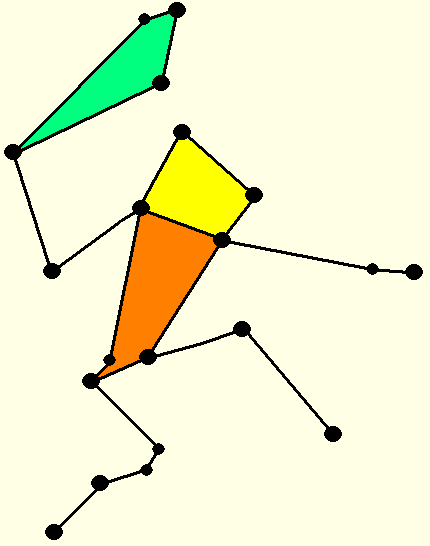
\includegraphics[scale=0.300000]{hercules-logo.png}}
\caption{HercuLeS, the constellation.}
\end{figure}

\phantomsection\label{contents}
\pdfbookmark[1]{Contents}{contents}
\tableofcontents



\section{1~~~HercuLeS basics%
  \label{hercules-basics}%
}


\subsection{1.1~~~Introduction%
  \label{introduction}%
}

HercuLeS is a \href{http://en.wikipedia.org/wiki/High-level_synthesis}{High-level synthesis} tool that automatically generates RTL VHDL
for non-programmable hardware. HercuLeS translates programs in NAC (a
bit-accurate typed-assembly language) to extended FSMDs (Finite-State Machines
with Datapath) in VHDL. HercuLeS can also be used for direct synthesis of ANSI C
code to VHDL with the help of a prototype translator from \href{http://gcc.gnu.org/wiki/GIMPLE}{GIMPLE} which is \href{http://gcc.gnu.org}{GCC}'s
new intermediate representation to NAC.

Internally, HercuLeS comprises of two main components: a frontend (nac2cdfg) and
a graph-based backend (cdfg2hdl):
%
\begin{description}
\item[{nac2cdfg}] \leavevmode 
translator from NAC (N-Address Code) IR, to flat CDFGs represented in \href{http://www.graphviz.org}{Graphviz}

\item[{cdfg2hdl}] \leavevmode 
the actual HLS tool for automatic FSMD hardware and self-checking testbench
generation from Graphviz files to VHDL

\end{description}

HercuLeS also has an additional ANSI C backend, allowing comparison of NAC
programs to reference ANSI C application code and the rapid prototyping of
applications (VHDL simulation can be slow depending on design complexity, input
data and the simulator used).

VHDL code generated by HercuLeS can be simulated with \href{http://ghdl.free.fr}{GHDL} and the industry-
standard \href{http://www.model.com}{Modelsim}. It is possible to generate VHDL using either the Synopsys
packages (the ``old'' de-facto standard) or the official IEEE library packages.
HercuLeS supports fixed-point arithmetic via \texttt{sfixed} and \texttt{ufixed}
vectors as defined by the \DUroletitlereference{VHDL-2008 fixed-point arithmetic packages}.
For this option, HercuLeS should be notified (via command-line option) to use
the IEEE packages.


\subsection{1.2~~~Conceptual flow%
  \label{conceptual-flow}%
}

The basic steps in the HercuLeS flow are shown in Fig. \hyperref[hercules-overview]{hercules-overview}.
C code is passed to GCC for GIMPLE dump generation, optionally following an
external source-level optimizer. Textual GIMPLE is then processed by
\emph{gimple2nac}; alternatively the user could directly supply a NAC translation
unit (TU).
\begin{figure}
\phantomsection\label{hercules-overview}
\noindent\makebox[\textwidth][c]{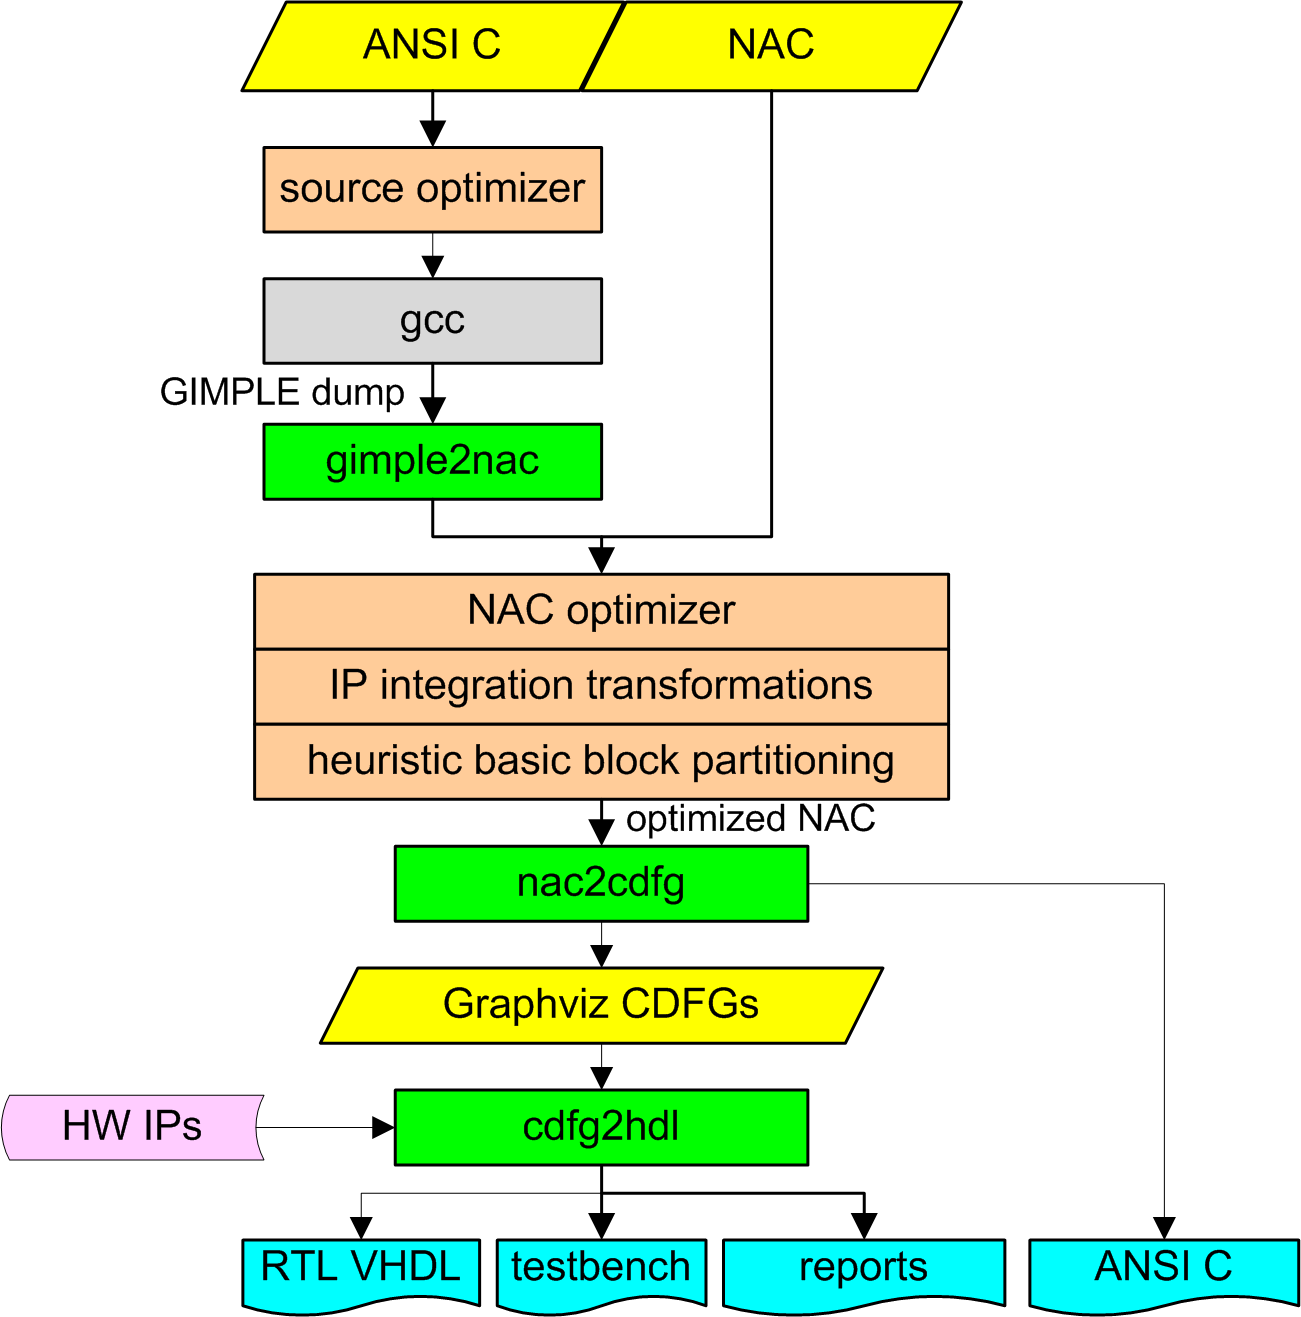
\includegraphics[scale=0.400000]{hercules-overview.png}}
\caption{The HercuLeS flow.}
\end{figure}

Various optimizations have been applied at the NAC level; peephole
transformations, if-conversion, and function call insertion to enable IP
integration. Heuristic basic block partitioning avoids the introduction of
excessive critical paths due to operation chaining.

The core of HercuLeS comprises of a frontend (\emph{nac2cdfg}) and a graph-based
backend (\emph{cdfg2hdl}). nac2cdfg is a translator from NAC to flat CDFGs
represented in \href{http://www.graphviz.org}{Graphviz}. cdfg2hdl is the actual synthesis kernel for
automatic FSMD hardware and self-checking testbench generation from Graphviz
CDFGs to VHDL.

nac2cdfg is used for parsing, analysis and CDFG extraction from NAC programs.
SSA form is supported based on minimal generation algorithms. Data flow
analysis uses on-demand graph reachability checking.

cdfg2hdl maps CDFGs to an extended FSMD MoC (Model of Computation).
For scheduling operations to specific states, either sequential or control-
aware ASAP scheduling can be used. ASAP can be combined with fast operation
chaining for better state workload balancing.

The generated FSMDs are generalized FSMs introducing embedded actions, with:
a) support of array input, output and streaming I/O ports,
b) communication with embedded block and distributed LUT memories,
c) latency-insensitive local interface between caller and callee FSMDs,
and d) interfacing to external IP blocks.

An additional ANSI C backend allows for rapid algorithm prototyping and NAC
verification. VHDL code can be simulated with \href{http://ghdl.free.fr}{GHDL} and \href{http://www.model.com}{Modelsim}.


\subsection{1.3~~~Overview%
  \label{overview}%
}

The current features of HercuLeS include:
%
\begin{itemize}

\item Multiple subprograms (procedures) and procedure calls

\item GIMPLE-to-NAC prototype frontend

\item NAC (N-address code) parsing and semantic analysis

\item Support for SSA form IR (in-to-SSA and out-of-SSA translations) based on
Appel's ``really-crude'' method and Aycock-Horspool's iteratively eliminating
algorithms for minimal SSA

\item Translation of NAC input programs to Graphviz CDFGs

\item CDFG (organized as Graphviz graphs) parsing and semantic analysis

\item Support of:
%
\begin{itemize}

\item multi-precision integer (std\_logic\_vector) and fixed-point (sfixed, ufixed)
arithmetic

\item basic low-level IR operators

\item extended FSMD model of computation

\item ``scalar'' and ``streamed'' (emitting a series of result values over time) outputs

\item single-dimensional arrays (Multidimensional arrays can always be reduced to
single-dimensional ones via matrix flattening)

\item parameter passing through array procedure arguments

\item automatic inference of block-RAM storage (for FPGAs)

\end{itemize}

\item Scheduling engines
%
\begin{itemize}

\item Sequential scheduling

\item Control-aware ASAP scheduling

\item Control-aware ASAP scheduling with operation chaining (2x-4x better
performance)

\end{itemize}

\item Optimizations
%
\begin{itemize}

\item Source-to-source C code optimizer (preliminary)

\item Integration of constant multiplication and division (\href{http://sourceforge.net/projects/kdiv}{kdiv}) optimizations

\item Integration of peephole-based optimizer

\item Data flow analysis (conservative custom method using on-demand graph
reachability checks)

\item Interface to a graph matching (graph and subgraph isomorphism) engine

\end{itemize}

\item Various APIs:
%
\begin{itemize}

\item Common abstract data types

\item Combinatorial objects generator

\item Interval arithmetic

\item Data flow analysis

\item Simple graphs (undirected and directed)

\item Attributed graphs (undirected and directed)

\end{itemize}

\item Generators
%
\begin{itemize}

\item VHDL design code (FSMD datapath and control)

\item Self-checking VHDL testbench

\item Various script files (Makefiles, shell scripts) for GHDL/Modelsim
simulations

\item Generation of Makefiles and scripts for running logic synthesis tools

\end{itemize}

\item Hardware operator library
%
\begin{itemize}

\item Configurable multipliers

\item Logarithm functions

\item Variable shifters

\item Dividers and modulo extractors

\end{itemize}

\item TODO list
%
\begin{itemize}

\item Multi-port memory synthesis

\item Access to global data from any procedure. Currently only the ``root''
procedure can access globals

\item Support of dynamically allocated data

\item Support of record data types (e.g. ANSI C structs)

\item Register optimization

\item List scheduling with operation chaining optimizations

\item Graph-based optimization engine

\item Enhanced data flow analysis

\item Recursive procedure support {[}\emph{Currently supported in the C backend}{]}

\end{itemize}

\end{itemize}


\subsection{1.4~~~Quick-start guide to the HercuLeS web interface%
  \label{quick-start-guide-to-the-hercules-web-interface}%
}

The purpose of this text is to provide a quick-start guide to using the HercuLeS
high-level synthesis tool through a web interface.
This version of HercuLeS does not provide access to certain features such as
arithmetic and loop-oriented optimizers.

Minimal requirements:
%
\begin{itemize}

\item Linux or Windows XP/Cygwin (a POSIX environment offering bash and common UNIX
utilities).

\item \href{http://ghdl.free.fr}{GHDL} or \href{http://www.model.com}{Modelsim}.

\end{itemize}
\newcounter{listcnt0}
\begin{list}{\arabic{listcnt0}.}
{
\usecounter{listcnt0}
\addtocounter{listcnt0}{-1}
\setlength{\rightmargin}{\leftmargin}
}

\item Visit the \href{http://www.nkavvadias.com/cgi-bin/herc.cgi}{HercuLeS web interface}.

\item Unzip \url{http://www.nkavvadias.com/hercules/hercules-contrib-vhdl.zip} to a local
directory, e.g. \texttt{C:\textbackslash{}hercules\textbackslash{}contrib}

\item Create an empty directory, e.g. \texttt{C:\textbackslash{}hercules\textbackslash{}tests}

\item Either select the supplied (already pasted) example of the ``fact'' (factorial)
function or copy and paste your own. Download \url{http://www.nkavvadias.com/hercules/small-examples.zip}
for a few ANSI C and NAC (generic assembly) code samples.

NOTES:
\newcounter{listcnt1}
\begin{list}{\alph{listcnt1}.}
{
\usecounter{listcnt1}
\setlength{\rightmargin}{\leftmargin}
}

\item In order to use the automatically-generated testbench, add a main() function
to your code, enclosed by the preprocessor directive:
\end{list}
\end{list}
%
\begin{quote}{\ttfamily \raggedright \noindent
\#ifdef~TEST\\
\#endif
}
\end{quote}
%
\begin{quote}
\setcounter{listcnt0}{0}
\begin{list}{\alph{listcnt0}.}
{
\usecounter{listcnt0}
\addtocounter{listcnt0}{1}
\setlength{\rightmargin}{\leftmargin}
}

\item In addition, it is expected that the main() function generates input and
reference output samples in hexadecimal format and in separate columns. A proper
main() would generate such samples in a file named fact\_test\_data.txt (for the
fact example).

\item Standard C library includes should be also enclosed by the aforementioned
directive.

\item Read Section 5 of \url{http://www.nkavvadias.com/hercules/hercules-web-guide.html}
for a short guide on ANSI C code style and limitations (WIP).
\end{list}

\end{quote}
\setcounter{listcnt0}{0}
\begin{list}{\arabic{listcnt0}.}
{
\usecounter{listcnt0}
\addtocounter{listcnt0}{3}
\setlength{\rightmargin}{\leftmargin}
}

\item On the web interface page, give the name of the top-level function/procedure
in your test code in the corresponding box. For instance, in the supplied
example this is:  \texttt{fact}

\item In the following box, give your personal email, e.g.
\href{mailto:nikolaos.kavvadias@gmail.com}{nikolaos.kavvadias@gmail.com}
Unless you provide an email address, it is not possible to receive generated
files from HercuLeS.

\item Choose implementation options from the menu or keep the defaults (where
multiple options exist, the first option is the default):
\setcounter{listcnt1}{0}
\begin{list}{\alph{listcnt1}.}
{
\usecounter{listcnt1}
\setlength{\rightmargin}{\leftmargin}
}

\item Input in ``C'' or ``NAC'' language.

\item Scheduling policy: sequential, ASAP or ASAP with chaining (could result in
faster hardware).

\item {[}Optional{]} Select visualization options, in case you want to receive the CDFG
and CFG visualizations of all processed functions/procedures.

\item Select the generation of simulation scripts for either ``GHDL'' or ``Modelsim''.

\item {[}Optional{]} Force the usage of block RAMs for ROM/RAM memory, when applicable.
\end{list}

\item Hit ``Submit''.

\item In a few minutes (depending on your input), you will receive the generated
files in your mailbox, archived in .tar.gz format.
Extract these files accordingly to a new subdirectory inside
\texttt{C:\textbackslash{}hercules\textbackslash{}tests}
For the case of the \texttt{fact} example this would be: \texttt{C:\textbackslash{}hercules\textbackslash{}tests\textbackslash{}fact}

\item From the command line (e.g. cygwin bash), change directory to
\texttt{C:\textbackslash{}hercules\textbackslash{}tests\textbackslash{}fact} and run the generated script that invokes the simulation:
\texttt{./fact.sh}

\item A successful simulation ends with an assertion reporting: ``Failure: NONE''.
Examine the diagnostic output in \DUroletitlereference{fact\_alg\_test\_results.txt} to obtain the number
of target hardware cycles needed to process each sample.
A simulation waveform is generated in file \DUroletitlereference{fact\_fsmd.vcd}.
Your design files are generated in VHDL (.vhd) using the IEEE libraries; for
the \texttt{fact} example this is: \texttt{fact.vhd}.
The automatically-generated testbench is named after the top-level function,
e.g. \texttt{fact\_tb.vhd}
\end{list}


\section{2~~~More on HercuLeS%
  \label{more-on-hercules}%
}


\subsection{2.1~~~How it works%
  \label{how-it-works}%
}

The following figure gives an internal view to the process flow of HercuLeS.
\begin{figure}
\noindent\makebox[\textwidth][c]{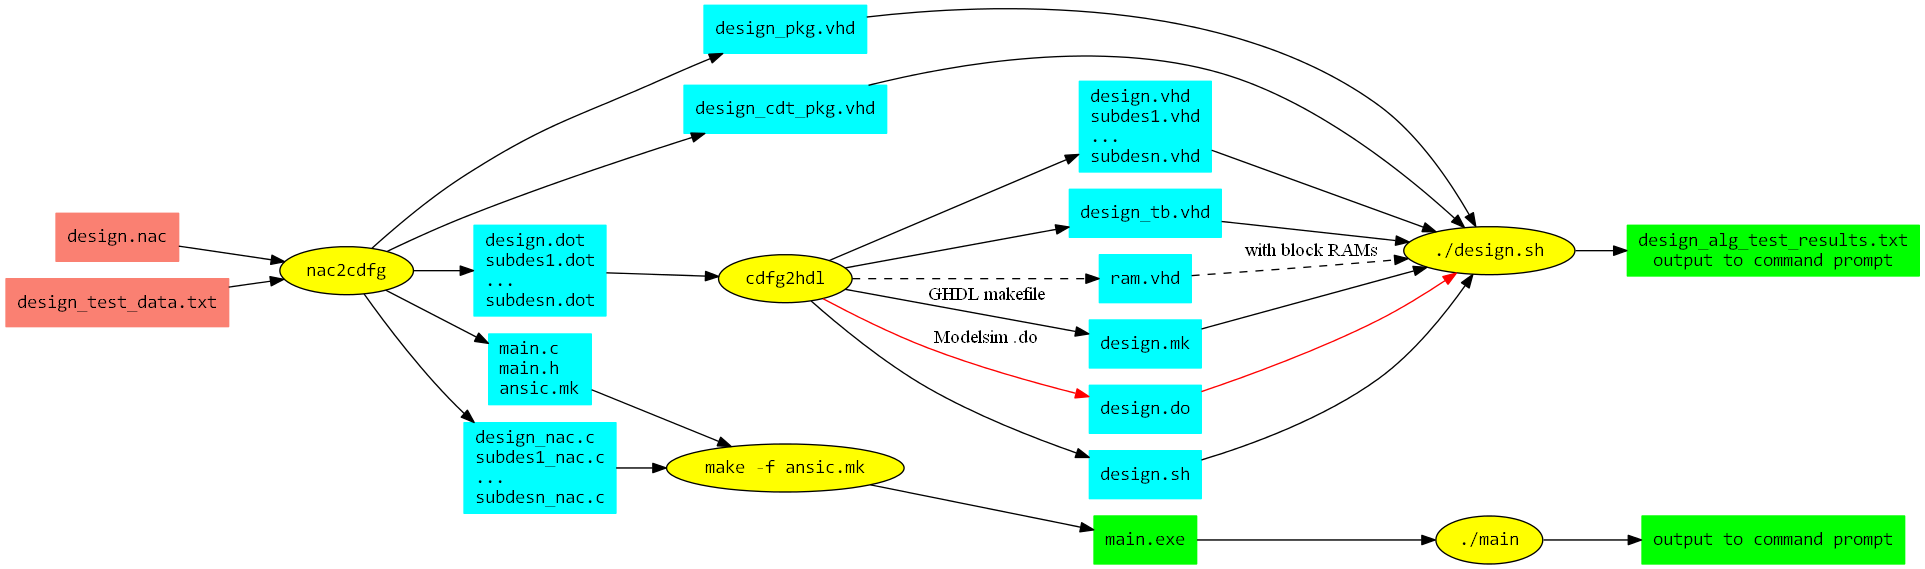
\includegraphics[scale=0.220000]{hlsflow.png}}
\caption{How HercuLeS works.}
\end{figure}

The user of HercuLeS must provide two input files:
%
\begin{itemize}

\item \DUroletitlereference{design.nac}: A NAC program translation unit providing the entire application.
The root procedure must be named ``design''.

\item \DUroletitlereference{design\_test\_data.txt}: Input/output reference values for use by the
automatically-generated testbench

\end{itemize}

Then, \emph{nac2cdfg} generates several files:
%
\begin{itemize}

\item \DUroletitlereference{design.dot, subdes1.dot, ..., subdesn.dot}: The Graphviz CDFGs for the root
procedure and all other procedures in the NAC program.

\item \DUroletitlereference{main.c, main.h, ansic.mk:} Files generated for running an ANSI C simulation.
\DUroletitlereference{ansic.mk} is an automatically-generated Makefile.

\item \DUroletitlereference{design\_nac.c, subdes1\_nac.c, ..., subdesn\_nac.c}: ANSI C backend files
providing C implementations of all procedures in the translation unit, generated
directly from NAC. They are used in the C simulations.

\item \DUroletitlereference{design\_pkg.vhd}: VHDL package incorporating the components for all NAC
procedures.

\item \DUroletitlereference{design\_cdt\_pkg.vhd}: VHDL package incorporating definitions of compound data
types (arrays).

\end{itemize}

Following this, there exist two possible flows; one for the generation and
simulation of synthesizable RTL VHDL for the NAC program, and one for a C
simulation.

The C simulation flow proceeds by invoking the \DUroletitlereference{ansic.mk} makefile by running:
%
\begin{quote}

\texttt{make -f ansic.mk}

\end{quote}

from the command line. This produces a \DUroletitlereference{main.exe} executable specification
(e.g. on Windows/Cygwin). Then, the executable is run:
%
\begin{quote}

\texttt{./main}

\end{quote}

and output is produced at the command prompt.

The VHDL flow involves processing all CDFG (.dot) files by \emph{cdfg2hdl}, the
actual backend tool of HercuLeS. cdfg2hdl generates several files:
%
\begin{itemize}

\item \DUroletitlereference{design.vhd, subdes1.vhd, ..., subdesn.vhd}: Synthesizable RTL VHDL for the
root procedure and all other procedures in the NAC program.

\item \DUroletitlereference{ram.vhd}: VHDL model of a dual-port synchronous read RAM for block RAM
inference. It is only used if block RAM mapping is enabled.

\item \DUroletitlereference{design\_tb.vhd}: The automatically-generated self-checking testbench.

\item \DUroletitlereference{design.mk}: Makefile for running a GHDL simulation.

\item \DUroletitlereference{design.do}: Modelsim do macro file for running a Modelsim simulation.

\item \DUroletitlereference{design.sh}: Bash shell script initiating either a GHDL or Modelsim
simulation.

\end{itemize}

Finally, the \DUroletitlereference{design.sh} script is run from the command line:
%
\begin{quote}

\texttt{./design.sh}

\end{quote}

This produces a text file (\DUroletitlereference{design\_alg\_test\_results.txt}) providing diagnostic
output from a simulation run. Output to the command prompt for any internal
program variable, procedure argument, etc can be produced by using the ``print''
NAC operation. A ``print'' is mapped to a VHDL ``assert'' construct or a C standard
library ``printf''.

Also, a VCD (\DUroletitlereference{design\_fsmd.vcd}) or GHW (\DUroletitlereference{design\_fsmd.ghw}) waveform file can be
generated for viewing with \href{http://sourceforge.net/projects/gtkwave}{GTKwave}. Windows binaries for GTKwave can be found
at \url{http://www.dspia.com/gtkwave.html}.


\subsection{2.2~~~nac2cdfg%
  \label{nac2cdfg}%
}

The usage of the \DUroletitlereference{nac2cdfg} is as follows:
%
\begin{quote}

\texttt{nac2cdfg {[}options{]} input.nac}

\end{quote}

where \texttt{options} is one or more of the following:
%
\begin{description}
\item[{-d:}] \leavevmode 
Enable debug output.

\item[{-force-data-types:}] \leavevmode 
Force predefined data types as given in NAC code. Essentially
disables the effect both interval analysis and the alternative
of using the unknown data type \texttt{na}.

\item[{-permissive:}] \leavevmode 
Allows non-strict forms and macrostatements of the NAC programming
language.

\item[{-ssa:}] \leavevmode 
Internal construction of SSA (Static Single Assignment) form.

\item[{-pseudo-ssa:}] \leavevmode 
Internal construction of local SSA-like form.

\item[{-use-appel:}] \leavevmode 
Enables SSA construction using Appel's algorithm.

\item[{-use-aycockhorspool:}] \leavevmode 
Enables SSA construction using the Aycock-Horspool algorithm (default).

\item[{-opt-spbb:}] \leavevmode 
Enables optimization 3 as discussed in the Aycock-Horspool paper,
which omits generating phi statements for single-predecessor BBs.
Supported only with -use-appel and -keep-ssa.

\item[{-keep-ssa:}] \leavevmode 
Does not perform out-of-SSA conversion and thus keeps PHI statements
in the generated CDFGs.

\item[{-limit-nacs:}] \leavevmode 
Limits the number of NACs in a translation unit to NAC\_LIMIT (about 25).

\item[{-emit-nac:}] \leavevmode 
Emit the equivalent NAC program after processing (including SSA
conversion, if enabled).

\item[{-emit-ansic:}] \leavevmode 
Emit the equivalent ANSI C program after processing (including SSA
conversion, if enabled).

\item[{-emit-cfg:}] \leavevmode 
Generate the Graphviz representations for all procedure CFGs.

\item[{-dump-varnum-nac:}] \leavevmode 
Dump the equivalent NAC program after SSA variable numbering.

\item[{-dump-phiins-nac:}] \leavevmode 
Dump the equivalent NAC program after SSA PHI insertion.

\item[{-dump-phimin-nac:}] \leavevmode 
Dump the equivalent NAC program after SSA PHI minimization.

\item[{-dump-phielm-nac:}] \leavevmode 
Dump the equivalent NAC program after SSA PHI elimination.

\item[{-dump-simdce-nac:}] \leavevmode 
Dump the equivalent NAC program after post-SSA dead code elimination.

\item[{-dump-tgf:}] \leavevmode 
Dump TGF (Trivial Graph Format) representations of program information.

\item[{-dump-arg:}] \leavevmode 
Dump ARG (attributed relational graph) representations of program information.

\item[{-dump-grh:}] \leavevmode 
Dump simple edge-list representations of program information.

\item[{-dump-poset:}] \leavevmode 
Dump poset (.p) file representations of program information.

\end{description}


\subsection{2.3~~~cdfg2hdl%
  \label{cdfg2hdl}%
}

The usage of the \DUroletitlereference{cdfg2hdl} is as follows:
%
\begin{quote}

\texttt{cdfg2hdl {[}options{]} input.dot}

\end{quote}

where \texttt{options} is one or more of the following:
%
\begin{description}
\item[{-d:}] \leavevmode 
Enable debug output (nothing yet).

\item[{-sched-<mode>:}] \leavevmode 
Perform scheduling on predefined acyclic regions.
Valid options for <mode>: \{sequential, asap, naive\}.

\item[{-mpint:}] \leavevmode 
Use multiple-precision arithmetic as implemented
by the public domain \href{http://stuff.mit.edu/afs/sipb/project/stk/src/STk-2.2.0/Mp/fgmp-1.0b5/}{fgmp} library.

\item[{-streaming:}] \leavevmode 
Generate code for hardware units with streaming
output(s), generating a sequence of values.

\item[{-vhd2vl:}] \leavevmode 
Generate code more friendly to the ``\href{http://doolittle.icarus.com/~larry/vhd2vl/}{vhd2vl}'' tool.

\item[{-use-rising-edge:}] \leavevmode 
Use calls to rising\_edge for clock event detection.

\item[{-use-component-pkg:}] \leavevmode 
Generate a package ``use'' for system-wide components.

\item[{-ghw:}] \leavevmode 
Generate a GHDL Waveform file (.ghw) after simulation.

\item[{-vcd:}] \leavevmode 
Generate a VCD waveform file (.vcd) after simulation.

\item[{-read-through, -read-first:}] \leavevmode 
Specify the mode for block RAM synchronous reads (default:
read-first).

\item[{-blockmem:}] \leavevmode 
Generate embedded block memories via inference.

\item[{-synopsys:}] \leavevmode 
Use the de-facto Synopsys IEEE library in the
generated design code (default).

\item[{-ieee:}] \leavevmode 
Use the normative IEEE library in the generated design code.

\item[{-hw-phis:}] \leavevmode 
Generate hardware for direct support of phi statements.

\item[{-fxp-trn-wrap:}] \leavevmode 
Support for fixed-point arithmetic with truncation
(quantization mode) and wrapping (overflow mode). This is
the default option.

\item[{-fxp-trn-sat:}] \leavevmode 
Support for fixed-point arithmetic with truncation
(quantization mode) and saturation (overflow mode).

\item[{-fxp-rnd-wrap:}] \leavevmode 
Support for fixed-point arithmetic with rounding
(quantization mode) and wrapping (overflow mode).

\item[{-fxp-rnd-sat:}] \leavevmode 
Support for fixed-point arithmetic with rounding
(quantization mode) and saturation (overflow mode).

\item[{-ghdl:}] \leavevmode 
Generate support files for GHDL simulation (default).

\item[{-mti:}] \leavevmode 
Generate support files for Modelsim simulation.

\item[{-quick-abort:}] \leavevmode 
Abort simulation immediately following the first error.

\end{description}


\subsubsection{2.3.1~~~CDFG construction%
  \label{cdfg-construction}%
}

A novel, fast CDFG construction algorithm has been devised for both SSA and
non-SSA NAC forms producing flat CDFGs as Graphviz files. A CDFG symbol table
item is a node (operation, procedure call, globalvar, or constant) or edge
(localvar) with user-defined attributes: the unique name, label and data type
specification; node and edge type enumeration; respective order of incoming or
outgoing edges; input/output argument order of a node and basic block index.
Further attributes can be defined, e.g. for scheduling bookkeeping.

This approach is unique since it focuses on building the CDFG symbol table (st)
from which the associated graph (cdfg) is constructed as one possible of many facets.
It naturally supports loop-carried dependencies and array accesses.
%
\begin{quote}{\ttfamily \raggedright \noindent
//~CDFG~construction~algorithm~accepting~BASIL~input.\\
NACtoCDFG()\\
~~input~List~BASILs,~List~variables,~List~labels,~Graph~cfg;\\
~~output~SymbolTable~st,~Graph~cdfg;\\
begin\\
~~Insert~constant,~input/output~arguments~and~globalvar\\
~~operand~nodes~to~st;\\
~~Insert~operation~nodes;\\
~~Insert~incoming~\{global/constant/input,~operation\}~and\\
~~outgoing~\{operation,~global/output\}~edges;\\
~~Add~control-dependence~edges~among~operation~nodes;\\
~~Add~data-dependence~edges~among~operation~nodes,\\
~~extract~loop-carried~dependencies~via~cfg-reachability;\\
~~Generate~cdfg~from~st;\\
end
}
\end{quote}


\section{3~~~gimple2nac%
  \label{gimple2nac}%
}

\emph{gimple2nac} translates GIMPLE dumps to NAC TUs, which presents challenges.
Currently, GIMPLE loses source semantics such as global scope variables.
A workaround for some cases is the definition of static variables in the
original source. Other issues involve: format inconsistencies following
different optimization passes, handling labels and array initialization
sequences, destroyed interfaces and lack of bit-accuracy. Some of these
problems are targeted by a GCC rewrite {[}\href{http://gcc.gnu.org/wiki/gimplebackend}{GIMPLEbe}{]} that will allow emitting
GIMPLE as a target language.


\subsection{3.1~~~Introduction%
  \label{id1}%
}

\emph{GIMPLE} is the machine-independent intermediate representation used in modern
GCC releases (post version 4.0). While the GIMPLE API for code generation and
manipulation has matured over time, the corresponding textual representation
is yet to be in a stable form. This issue hampers many serious efforts for
code generation from and to GIMPLE.

Good candidates for the textual representation seem to have been in play for
some time. The wiki site \url{http://gcc.gnu.org/wiki/GIMPLE} sketches the textual
IR that is expected to be implemented by the GIMPLE frontend and backend
(both under development). Another case of a textual GIMPLE are the formats
generated as a \emph{GIMPLE dumps}. We distinguish here two formats: the format
in *.t004.gimple files (\emph{tagged} GIMPLE) and the one e.g. in *.t140.optimized
files (\emph{GIMPLE-C}). Both formats express the low-level GIMPLE representation,
which is closer to classic three-address code than high-level GIMPLE; the latter
is closer to the GENERIC AST representation. An extended form of GIMPLE dumps
are expected to be established as the GIMPLE language semantics.

For reference tagged GIMPLE is generated by the command-line option:
%
\begin{quote}

\texttt{-fdump-tree-all-raw}

\end{quote}

while GIMPLE-C is generated by:
%
\begin{quote}

\texttt{-fdump-tree-all} and \texttt{-fdump-tree-gimple}

\end{quote}

the latter only emitting the *.t004.gimple file.

The rest of this document discusses open issues with the textual GIMPLE IRs,
focusing on the tagged GIMPLE format. It will not cover extended semantics
issues that are covered much better at \url{http://gcc.gnu.org/wiki/GIMPLEFrontEnd}


\subsection{3.2~~~Target audience%
  \label{target-audience}%
}

This section is expected to be of interest to compiler/translator implementors
using GIMPLE as either a source or target language.


\subsection{3.3~~~Issues with tagged GIMPLE%
  \label{issues-with-tagged-gimple}%
}

Here follows a listing of some issues that can be identified with using tagged
GIMPLE. Most of them apply to the GIMPLE-C format as well.


\subsubsection{3.3.1~~~Losing the original semantics of the source program%
  \label{losing-the-original-semantics-of-the-source-program}%
}

One such example is the omission of emitting global variables. A workaround
for some cases is the definition of static variables in the original source.
This approach provides only specific file/translation unit scope to globals
but it is not certain whether the extern specifier is handled properly for
referencing these globals from external scope.


\subsubsection{3.3.2~~~Inconsistency in handling labels%
  \label{inconsistency-in-handling-labels}%
}

Automatically generated labels (by the gimplifier) and labels defined in the
source program are represented differently. The first category are enclosed
in single wedges \texttt{< >} while the later are explicitly defined and are
used without wedges.

For example, this is the definition of an automatically generated label:
%
\begin{quote}

\texttt{gimple\_label <{}<D.1983>{}>}

\end{quote}

while the following is the (redundant) definition:
%
\begin{quote}

\texttt{void V1 = <{}<{}< error >{}>{}>;
...
`{}`gimple\_label <V1>}

\end{quote}

and the use of a source label:
%
\begin{quote}

\texttt{gimple\_cond <eq\_expr, D.1985, 1, V5, <D.1986>{}>}

\end{quote}


\subsubsection{3.3.3~~~Destroyed interfaces%
  \label{destroyed-interfaces}%
}

Function interfaces are not maintained appropriately since the original
argument types in a function definition may be replaced. This is the case
with array arguments (with static sizes) in the definition of non-root
procedures.

Here follows an example. This is the a partial view of the source program:
%
\begin{quote}{\ttfamily \raggedright \noindent
void~evalcoins(int~n,~int~amount,~int~C{[}{]},~int~*ncoins,~int~D{[}{]})\\
\{\\
~~...\\
\}\\
~\\
void~coins(int~n\_eurocents,~int~*n\_coins\_used)\\
\{\\
~~int~C\_euro{[}15{]},~D\_euro{[}15{]};\\
~~...\\
~~evalcoins(15,~n\_eurocents,~C\_euro,~\&n\_items,~D\_euro);\\
~~...\\
\}\\
~\\
However,~this~is~the~tagged~GIMPLE~form~of~the~same~program:
}
\end{quote}
%
\begin{quote}{\ttfamily \raggedright \noindent
evalcoins~(int~n,~int~amount,~int~*~C,~int~*~ncoins,~int~*~D)\\
gimple\_bind~<\\
~~...\\
>\\
~\\
coins~(int~n\_eurocents,~int~*~n\_coins\_used)\\
gimple\_bind~<\\
~~int~C\_euro{[}15{]};\\
~~int~D\_euro{[}15{]};\\
~~...\\
~~gimple\_call~<evalcoins,~NULL,~15,~n\_eurocents,\\
~~~~~~~~~~~~~~~\&C\_euro{[}0{]},~\&n\_items,~\&D\_euro{[}0{]}>\\
~~...\\
>
}
\end{quote}


\subsubsection{3.3.4~~~Pointer expressions%
  \label{pointer-expressions}%
}

Low-level GIMPLE (tagged and GIMPLE-C) use two basic specific operations for
dealing with pointer expressions and indirect references, the
\texttt{pointer\_plus\_expr} and \texttt{indirect\_ref}.

A \texttt{pointer\_plus\_expr} in tagged GIMPLE appears as follows:
%
\begin{quote}

\texttt{gimple\_assign<pointer\_plus\_expr, D.1986, D, D.1985>}

\end{quote}

where D is an array, D.1985 a temporary int variable and D.1986 a temporary
variable defined as pointer to int.

The same in GIMPLE-C is the following:
%
\begin{quote}

\texttt{D.1986 = D + D.1985}

\end{quote}

This operation adds the offset determined by D.1985 to the base address of array
D, expressed as D. Pointer D.1986 then can be used for intexing the array.

A typical idiom in generated GIMPLE suggests that \texttt{pointer\_plus\_expr} is
followed by an \texttt{indirect\_ref}. The indirect reference is used to access
the array and loading the contents of a memory position to a variable.

An \texttt{indirect\_ref} in tagged GIMPLE appears as follows:
%
\begin{quote}

\texttt{gimple\_assign<indirect\_ref, D.1987, *D.1986, NULL>}

\end{quote}

and the same in GIMPLE-C is:
%
\begin{quote}

\texttt{D.1987 = *D.1986;}

\end{quote}

In order to avoid a thorough pointer analysis for establishing that
D.1986 points to the contents of array D, typical data-dependence
analysis can be used to trace that D is the referenced entity by D.1986.


\subsubsection{3.3.5~~~Function calls%
  \label{function-calls}%
}

Function calls are represented by \texttt{gimple\_call} in tagged GIMPLE. Due to
the issue 3 (Destroyed interfaces), in some cases calls-by-reference
appear when not really needed. This refers to the simulated call-by-reference
available in the C programming language, and not the actual kind that can
be found, e.g. in Perl.

For example the following call is by-reference:
%
\begin{quote}

\texttt{gimple\_call <..., \&C\_euro{[}0{]},...>}

\end{quote}

making use of the address of the first element of C\_euro (the base address).

With interfaces kept unchanged, the following would suffice:
%
\begin{quote}

\texttt{gimple\_call <..., C\_euro, ...>}

\end{quote}


\subsubsection{3.3.6~~~Inconsistency in array initialization sequences%
  \label{inconsistency-in-array-initialization-sequences}%
}

An array can be initialized either by a literal initialization list or
by emitting a sequence of operations for initializing its contents.
From a black-box point of view, it seems that the gimplifier arbitrarily
chooses which approach to follow.

For example, in our example, the C\_euro is initialized via explicit
operations:
%
\begin{quote}{\ttfamily \raggedright \noindent
gimple\_assign~<integer\_cst,~C\_euro{[}0{]},~1,~NULL>\\
gimple\_assign~<integer\_cst,~C\_euro{[}1{]},~2,~NULL>\\
gimple\_assign~<integer\_cst,~C\_euro{[}2{]},~5,~NULL>\\
gimple\_assign~<integer\_cst,~C\_euro{[}3{]},~10,~NULL>\\
gimple\_assign~<integer\_cst,~C\_euro{[}4{]},~20,~NULL>\\
gimple\_assign~<integer\_cst,~C\_euro{[}5{]},~50,~NULL>\\
gimple\_assign~<integer\_cst,~C\_euro{[}6{]},~100,~NULL>\\
gimple\_assign~<integer\_cst,~C\_euro{[}7{]},~200,~NULL>\\
gimple\_assign~<integer\_cst,~C\_euro{[}8{]},~500,~NULL>\\
gimple\_assign~<integer\_cst,~C\_euro{[}9{]},~1000,~NULL>\\
gimple\_assign~<integer\_cst,~C\_euro{[}10{]},~2000,~NULL>\\
gimple\_assign~<integer\_cst,~C\_euro{[}11{]},~5000,~NULL>\\
gimple\_assign~<integer\_cst,~C\_euro{[}12{]},~10000,~NULL>\\
gimple\_assign~<integer\_cst,~C\_euro{[}13{]},~20000,~NULL>\\
gimple\_assign~<integer\_cst,~C\_euro{[}14{]},~50000,~NULL>\\
~\\
It~is~not~clear~why~an~initialization~list~is~not~used:
}
\end{quote}
%
\begin{quote}{\ttfamily \raggedright \noindent
int~C\_euro{[}15{]}~=~\{1,~2,~5,~10,~20,~50,\\
~~~~~~~~~~~~~~~~~~100,~200,~500,~1000,~2000,~5000,\\
~~~~~~~~~~~~~~~~~~10000,~20000,~50000\};
}
\end{quote}

Automatically generated labels (by the gimplifier) and labels defined in the
source program are represented differently. The first category are enclosed
in single wedges \texttt{< >} while the later are explicitly defined and are
used without wedges.

For example, this is the definition of an automatically generated label:
%
\begin{quote}

\texttt{gimple\_label <{}<D.1983>{}>}

\end{quote}

while the following is the (redundant) definition:
%
\begin{quote}

\texttt{void V1 = <{}<{}< error >{}>{}>;
...
`{}`gimple\_label <V1>}

\end{quote}

and the use of a source label:
%
\begin{quote}

\texttt{gimple\_cond <eq\_expr, D.1985, 1, V5, <D.1986>{}>}

\end{quote}


\subsubsection{3.3.7~~~Inconsistency of the tagged GIMPLE format%
  \label{inconsistency-of-the-tagged-gimple-format}%
}

As discussed in the introduction, the tagged GIMPLE format uses alternate
syntax for the unoptimized (*.t004.gimple) and certain optimized (e.g.
*.t140.gimple) intermediate code dumps. It would be clearer if a single
convention throughout all GIMPLE dumps.


\subsubsection{3.3.8~~~Lack of bit-accurate semantics%
  \label{lack-of-bit-accurate-semantics}%
}

The availability of bit-accurate data types is an interesting asset of
modern compiler infrastructures such as LLVM: \url{http://www.llvm.org}. LLVM
uses the LLVM bitcode IR which adheres to such semantics. On the other
side, GCC GIMPLE might be too closely coupled with C-like semantics.
Especially, implementors of non-conventional backend architectures
(e.g. developers of hardware compilers) would be interested in a form of
GIMPLE with bit-accurate types.

For example, the following would denote a 14-bit unsigned integer
and a 8.16 signed fixed-point representation, respectively.
%
\begin{quote}
%
\begin{itemize}

\item \texttt{u14}

\item \texttt{q8.16s}

\end{itemize}

\end{quote}


\subsection{3.4~~~Final notes on GIMPLE%
  \label{final-notes-on-gimple}%
}

This section is a work-in-progress. Several aspects of programming language
translation to low-level GIMPLE are not covered:
\setcounter{listcnt0}{0}
\begin{list}{\arabic{listcnt0}.}
{
\usecounter{listcnt0}
\setlength{\rightmargin}{\leftmargin}
}

\item Support for recursion.

\item OMP semantics.

\item \texttt{\_Bool} data types.

\item Explicit return types (other than void).

\item Semantics expected to be integrated as part of GCC mainline. These reflect
the current status of the \texttt{gimple-front-end} branch, which adds important
capabilities to the GIMPLE infrastructure such as consistently-styled
declarations for pointers, arrays, and compound types (structs, unions).
\end{list}


\section{4~~~The NAC programming language%
  \label{the-nac-programming-language}%
}


\subsection{4.1~~~Introduction%
  \label{id2}%
}

NAC (N-Address Code) is the name of a simplistic imperative programming language
with light semantics devised by Nikolaos Kavvadias. Its main use is as an
executable/interpretable intermediate representation for compilation frameworks
(compilers, high-level synthesis tools, etc).

NAC statements are either labels, n-address instructions or procedure calls.

A label is formatted as follows:
%
\begin{itemize}

\item label:

\end{itemize}

An n-address instruction is actually the specification of a mapping from
a set of n ordered inputs to a set of m ordered outputs. An n-address
instruction (or else termed as an \{m, n\}-NAC) is formatted as follows:
%
\begin{itemize}

\item \texttt{outp1, ..., outpm <= operation inp1, ..., inpn;}

\end{itemize}

where
%
\begin{itemize}

\item \emph{operation} is a mnemonic referring to an IR-level instruction

\item \emph{outp1}, ..., \emph{outpm} are the m outputs of the instruction

\item \emph{inp1}, ..., \emph{inpn} are the n inputs of the instruction

\end{itemize}

Similarly, a procedure call, which is a non-atomic operation is formatted
as follows, in order to distinguished from an atomic operation:
%
\begin{itemize}

\item \texttt{(outp1, ..., outpm) <= procedure-name (inp1, ..., inpn);}

\end{itemize}

where
%
\begin{itemize}

\item \emph{procedure-name} is the name of called procedure.

\end{itemize}

For a procedure without input and output arguments, the following notation
is used to distinguish it from an atomic operation with no arguments:
%
\begin{itemize}

\item \texttt{() <= procedure-name ();}

\end{itemize}

NAC is a typed language. Data type specifications are essentially strings that
can be easily decoded by a regular expression scanner. All declared objects
(global variables, constants, local variables, input and output procedure
arguments) have a type specification. Data types in NAC are classified in the
following categories:
%
\begin{itemize}

\item UNSIGNED\_INTEGER denoted as U<num>: {[}Uu{]}{[}0-9{]}+

\item SIGNED\_INTEGER denoted as S<num>: {[}Ss{]}{[}0-9{]}+

\item Fixed-point numbers are denoted as Q<ipart>.F<ipart>{[}S|U{]}: Q{[}0-9{]}+.{[}0-9{]}+{[}S|U{]},
with ipart being the integer part and fpart the fractional part of the number.
SIGNED\_FIXED\_POINT uses the \DUroletitlereference{S} suffix, whereas UNSIGNED\_FIXED\_POINT uses the
\DUroletitlereference{U} suffix, correspondingly

\item FLOATING\_POINT denoted as F<spart>.<epart>.<mpart>: F{[}0|1{]}.{[}0-9{]}+.{[}0-9{]}+,
with spart being the sign, epart the exponent and mpart the mantissa of the
number

\item RATIONAL (no consistent format yet)

\item CONTINUED\_FRACTION (no consistent format yet)

\end{itemize}

As of 2010-11-29, there is initial support for the SIGNED\_FIXED\_POINT and
UNSIGNED\_FIXED\_POINT data types. As of 2012-02-23 there is also initial
support (for the C backend) for the FLOATING\_POINT data types, especially
the IEEE-754 compliant ``single'' and ``double''. Support for UNSIGNED\_INTEGER
and SIGNED\_INTEGER data types is considered mature.

In NAC parlance, the following keywords are used:
%
\begin{description}
\item[{\texttt{globalvar}}] \leavevmode 
a global scalar or single-dimensional array variable. An array
variable is permitted to have an optional numerical initialization. A scalar
variable is assumed to be initialized to zero.

\item[{\texttt{localvar}}] \leavevmode 
a local scalar or single-dimensional array variable. This variable
is only visible within the procedure. Again, an array variable is permitted to
have an optional numerical initialization. A scalar variable is assumed to be
initialized to zero.

\item[{\texttt{in}}] \leavevmode 
an input argument to the given procedure.

\item[{\texttt{out}}] \leavevmode 
an output argument to the given procedure.

\end{description}

Please note that the use of \texttt{constant} (declaration of a globally-visible
constant value) has been discontinued and will not be supported in the
future.


\subsection{4.2~~~NAC instructions%
  \label{nac-instructions}%
}

The NAC programming language is extensible, meaning that the grammar accepts
user-specific instruction mnemonics.

A common set of NAC instructions is listed below, along with the corresponding
format and description.

No-operation: \texttt{nop}
%
\begin{quote}

\texttt{nop;}

Performs no action at all.

\end{quote}

Move operand: \texttt{mov}
%
\begin{quote}

\texttt{dst1 <= mov src1;}

Copy the contents of operand src1 to dst1.

\end{quote}

Load constant: \texttt{ldc}
%
\begin{quote}

\texttt{dst1 <= ldc cnst1;}

Copy the value of cnst1 to operand dst1.

\end{quote}

Unconditional jump: \texttt{jmpun}
%
\begin{quote}

\texttt{S\_dst1 <= jmpun;}

Jump to label \texttt{S\_dst1}.

\end{quote}

Conditional jump: \texttt{jmpeq}, jmpne``, \texttt{jmplt}, jmple``, \texttt{jmpgt}, jmpge``
%
\begin{quote}

\texttt{S\_TRGT, S\_TRGF <= jmpzz src1, src2;}

where:
%
\begin{itemize}

\item \texttt{zz} can be one of the following:
%
\begin{itemize}

\item eq: jump if equal

\item ne: jump if not equal

\item lt: jump if less than

\item le: jump if less than or equal

\item gt: jump if greater than

\item ge: jump if greater than or equal

\end{itemize}

\item src1, src2 are the instruction source operands

\item S\_TRGT, S\_TRGF, are the target addresses for a true and false condition,
respectively

\end{itemize}

\end{quote}

Binary logical instructions: \texttt{and}, \texttt{ior}, \texttt{xor}, \texttt{nand}, \texttt{nor}, \texttt{xnor}
%
\begin{quote}

\texttt{dst1 <= <mnemonic> src1, src2;}

where:
%
\begin{itemize}

\item mnemonic can be one of the following:
%
\begin{itemize}

\item and: Logical AND

\item ior: Logical inclusive-OR

\item xor: Logical exclusive-OR

\item nand: Logical NAND

\item nor: Logical NOR

\item xnor: Logical XNOR

\end{itemize}

\item src1, src2 are the source operands

\item dst1 is the destination operand

\end{itemize}

\end{quote}

Unary logical instruction: \texttt{not}
%
\begin{quote}

\texttt{dst1 <= not src1;}

Copy the 1's-complement of operand src1 to dst1.

\end{quote}

Binary arithmetic instructions: \texttt{add}, \texttt{sub}
%
\begin{quote}

\texttt{dst1 <= mnemonic src1, src2;}

where:
%
\begin{itemize}

\item mnemonic can be one of the following:
%
\begin{itemize}

\item add: 2's-complement addition

\item sub: 2's-complement subtraction

\end{itemize}

\item src1, src2 are the source operands

\item dst1 is the destination operand

\end{itemize}

\end{quote}

Unary arithmetic instructions: \texttt{neg}
%
\begin{quote}

\texttt{dst1 <= neg src1;}

Copies the negated version of src1 to dst1.

\end{quote}

Quaternary multiplexing instruction: \texttt{mux}
%
\begin{quote}

\texttt{dst1 <= muxzz src1, src2, src3, src4;}

where:
%
\begin{itemize}

\item zz can be one of the following:
%
\begin{itemize}

\item eq: jump if equal

\item ne: jump if not equal

\item lt: jump if less than

\item le: jump if less than or equal

\item gt: jump if greater than

\item ge: jump if greater than or equal

\end{itemize}

\item src1, src2, are the source operands compared: \texttt{if (src1 zz src2)}

\item src3 is the copy operand when the comparison evaluates to TRUE

\item src4 is the copy operand when the comparison evaluates to FALSE

\item dst1 is the destination operand

\item NOTE: A \texttt{muxzz} is equivalent to the following C code:

\end{itemize}

\end{quote}
%
\begin{quote}{\ttfamily \raggedright \noindent
if~(src1~zz~src2)~\{~//~zz:~"==",~"!=",~"<",~"<=",~">",~or~">="\\
~~dst1~=~src3;\\
\}~else~\{\\
~~dst1~=~src4;\\
\}
}
\end{quote}

Set on comparison instruction: \texttt{set}
%
\begin{quote}

\texttt{dst1 <= setzz src1, src2;}

where:
%
\begin{itemize}

\item zz can be one of the following:
%
\begin{itemize}

\item eq: jump if equal

\item ne: jump if not equal

\item lt: jump if less than

\item le: jump if less than or equal

\item gt: jump if greater than

\item ge: jump if greater than or equal

\end{itemize}

\item src1, src2, are the source operands compared: \texttt{src1 zz src2}

\item src3 is the copy operand when the comparison evaluates to TRUE

\item src4 is the copy operand when the comparison evaluates to FALSE

\item dst1 is the destination operand (gets a value either 0 or 1).

\item NOTE: A \texttt{setzz} is equivalent to the following C code:

\end{itemize}

\end{quote}
%
\begin{quote}{\ttfamily \raggedright \noindent
`{}`dst1~=~(src1~zz~src2);~//~zz:~"==",~"!=",~"<",~"<=",~">",~or~">="
}
\end{quote}

Complex unary arithmetic instructions: \texttt{abs}
%
\begin{quote}

\texttt{dst1 <= abs src1;}

Copies the absolute value of src1 to dst1.

\end{quote}

Complex binary arithmetic instructions: \texttt{max}, \texttt{min}
%
\begin{quote}

\texttt{dst1 <= mnemonic src1, src2;}

where:
%
\begin{itemize}

\item mnemonic can be one of the following:
%
\begin{itemize}

\item max: Assign the maximum of src1 and src2 to dst1

\item min: Assign the minimum of src1 and src2 to dst1

\end{itemize}

\item src1, src2 are the source operands

\item dst1 is the destination operand

\end{itemize}

\end{quote}

Shift instructions: \texttt{shl}, \texttt{shr}
%
\begin{quote}

\texttt{dst1 <= mnemonic src1, src2;}

where:
%
\begin{itemize}

\item mnemonic can be one of the following:
%
\begin{itemize}

\item shl: Logical left shift of src1 by the amount stored in src2, with
the result copied to dst1

\item shr: Either logical or arithmetic (depending on the operand data types)
shift of src1 by the amount stored in src2, with the result copied to
dst1

\end{itemize}

\item src1, src2 are the source operands

\item dst1 is the destination operand

\end{itemize}

\end{quote}

Rotate instructions: \texttt{rotl}, \texttt{rotr}
%
\begin{quote}

\texttt{dst1 <= mnemonic src1, src2;}

where:
%
\begin{itemize}

\item mnemonic can be one of the following:
%
\begin{itemize}

\item rotl: Left rotation of the value of src1 by the amount stored in src2,
with the result copied to dst1

\item rotr: Right rotation of the value of src1 by the amount stored in src2,
with the result copied to dst1

\end{itemize}

\item src1, src2 are the source operands

\item dst1 is the destination operand

\end{itemize}

\end{quote}

Multiplication instructions: \texttt{mul}
%
\begin{quote}

\texttt{dst1 <= mul src1, src2;}

Multiplies the contents of src1 and src2 and copies the (possibly truncated)
result to dst1.

\end{quote}

Combined division-modulus instructions: \texttt{divrem}
%
\begin{quote}

\texttt{dst1, dst2 <= divrem src1, src2;}

Divides the contents of src1 and src2 and copies the quotient to dst1 and
the remainder to dst2.

\end{quote}

Division instructions: \texttt{div}, \texttt{rem}
%
\begin{quote}

\texttt{dst1 <= mnemonic src1, src2;}

where:
%
\begin{itemize}

\item mnemonic can be one of the following:
%
\begin{itemize}

\item div: Divides the contents of src1 and src2 and copies the quotient to
dst1

\item rem: Divides the contents of src1 and src2 and copies the remainder to
dst1

\end{itemize}

\item src1, src2 are the source operands

\item dst1 is the destination operand

\end{itemize}

\end{quote}

Data type/bitwidth conversion instructions: \texttt{zxt}, \texttt{sxt}, \texttt{trunc}
%
\begin{quote}

\texttt{dst1 <= mnemonic src1;}

where:
%
\begin{itemize}

\item mnemonic can be one of the following:
%
\begin{itemize}

\item zxt: Zero-extends src1 to the (larger) bitwidth of dst1

\item sxt: Sign-extends src1 to the (larger) bitwidth of dst1

\item trunc: Truncates src1 to the (smaller) bitwidth of dst1

\end{itemize}

\item src1 is the source operand

\item dst1 is the destination operand

\end{itemize}

\end{quote}

Bit manipulation instructions: \texttt{bitins}, \texttt{bitext}
%
\begin{quote}

\texttt{dst1 <= mnemonic src1, src2, src3;}

where:
%
\begin{itemize}

\item mnemonic can be one of the following:
%
\begin{itemize}

\item bitins: Insert a bitvector denoted by the downto range {[}src2..src3{]} of src1
to dst1

\item bitext: Extract a bitvector denoted by the downto range {[}src2..src3{]} from
src1 and assign it to dst1

\end{itemize}

\item src1 is the source operand

\item src2 are two source operands (constant or variables) that denote the downto
range. The runtime numerical value of src2 must be larger or equal to src3,
and within the range of dst1

\item dst1 is the destination operand

\end{itemize}

These instructions define bitfield insertion and extraction primitives. They
can also be defined for fixed-point operands given additional constraints.

\end{quote}

Load variable from array: \texttt{load}
%
\begin{quote}

\texttt{dst1 <= load src1, src2;}

Loads the contents of array src1 from the absolute address src2 to the
variable dst1.

\end{quote}

Store variable to array: \texttt{store}
%
\begin{quote}

\texttt{dst1 <= store src1, src2;}

Stores the value of variable src1 to address src2 of array dst1.

\end{quote}


\subsubsection{4.2.1~~~Fixed-point operators%
  \label{fixed-point-operators}%
}

The use of fixed-point arithmetic provides an inexpensive means for improved
numerical dynamic range, when artifacts due to quantization and overflow effects
can be tolerated. Rounding operators are used for controlling the numerical
precision involved in a series of computations; they are defined for
inexact arithmetic representations such as fixed- and floating-point.
Proposed and in-use specifications for fixed-point arithmetic of
related practice include C99 and the Mentor ACDT (Algorithmic C Data Types).

Fixed-point arithmetic is a variant of the typical integral representation
(2's-complement signed or unsigned) where a binary point is defined, purely
as a notational artifact to signify integer powers of 2 with a negative exponent.
Assuming an integer part of width \texttt{IW > 0} and a fractional part with
\texttt{-FW < 0}, the VHDL-2008 \texttt{sfixed} data type has a range of
\texttt{2\textasciicircum{}\{IW-1\}-2\textasciicircum{}\{|FW|\}} to \texttt{-2\textasciicircum{}\{IW-1\}} with a representable quantum of
\texttt{2\textasciicircum{}|FW|}. The corresponding \texttt{ufixed} type has the following range:
\texttt{2\textasciicircum{}\{IW\}-2\textasciicircum{}\{|FW|\}} to \texttt{0}. Both are defined properly given a \texttt{{[}IW-1:-FW{]}}
vector range.

This is a proposed list of extension operators for use with
fixed-point variables support in the NAC programming language.

Conversion from integer to fixed-point format: \texttt{i2ufx}, \texttt{i2sfx}
%
\begin{quote}

\texttt{dst1 <= i2zfx src1;}

where:
%
\begin{itemize}

\item \texttt{z} can be one of the following:
%
\begin{itemize}

\item u: conversion to the ufixed (UNSIGNED\_FIXED\_POINT) format

\item s: conversion to the sfixed (SIGNED\_FIXED\_POINT) format

\end{itemize}

\item src1 is the source operand

\item dst1 is the destination operand

\end{itemize}

Converts an integer to a fixed-point number without loss of precision.

\end{quote}

Conversion from fixed-point to integer format: \texttt{ufx2i}, \texttt{sfx2i}
%
\begin{quote}

\texttt{dst1 <= zfx2i src1;}

where:
%
\begin{itemize}

\item \texttt{z} can be one of the following:
%
\begin{itemize}

\item u: conversion to the ufixed (UNSIGNED\_FIXED\_POINT) format

\item s: conversion to the sfixed (SIGNED\_FIXED\_POINT) format

\end{itemize}

\item src1 is the source operand

\item dst1 is the destination operand

\end{itemize}

Converts a fixed-point number to an integer. In case of a non-zero fractional part
of the fixed-number, truncation occurs. The type of the integer result (UNSIGNED\_INTEGER
or SIGNED\_INTEGER) must be compatible to the type of the fixed-point input argument
to assure a proper conversion.

\end{quote}

Resize instruction: \texttt{resize}
%
\begin{quote}

\texttt{dst1 <= resize src1, src2, src3;}

where:
%
\begin{itemize}

\item src1 is the source fixed-point operand

\item src2, src3 are numerical values (integers) that denote the new size (high-to-low range)
of the resulting fixed-point operand

\item dst1 is the destination fixed-point operand

\end{itemize}

\end{quote}

Fixed-point rounding instructions: \texttt{ceil}, \texttt{fix}, \texttt{floor}, \texttt{round}, \texttt{nearest}, \texttt{convergent}
%
\begin{quote}

\texttt{dst1 <= mnemonic src1;}

where:
%
\begin{itemize}

\item src1 is the source operand

\item dst1 is the destination operand

\end{itemize}

These operations are used to performing rounding of fixed-point operands with
different criteria. They emulate the behavior of corresponding MATLAB intrinsic
functions. Rounding behavior is summarized as follows:
%
\begin{itemize}

\item ceil: round towards plus infinity.

\item fix: round towards zero.

\item floor: round towards minus infinity.

\item round: round to nearest; ties to greatest absolute value.

\item nearest: round to nearest; ties to plus infinity.

\item convergent: round to nearest; ties to closest even.

\end{itemize}

\end{quote}


\subsection{4.3~~~Macroinsructions%
  \label{macroinsructions}%
}

For simplifying programming in the NAC language, a set of macroinstructions
are available:

A) Automatic replacement of incomplete conditional jumps:
The pattern
%
\begin{quote}

\begin{DUlineblock}{0em}
\item[] \texttt{S\_TRUE <= jmpxx opnd1, opnd2;}
\end{DUlineblock}

\end{quote}

is replaced by:
%
\begin{quote}

\begin{DUlineblock}{0em}
\item[] \texttt{S\_TRUE, S\_FALSE <= jmpxx opnd1, opnd2;}
\item[] \texttt{S\_FALSE:}
\end{DUlineblock}

\end{quote}

Label \texttt{S\_FALSE} is generated only if it doesn't already exist.

B) Addition of ``forgotten'' unconditional jumps. The pattern:
%
\begin{quote}

\begin{DUlineblock}{0em}
\item[]
\begin{DUlineblock}{\DUlineblockindent}
\item[] \texttt{no-jump-instruction;}
\end{DUlineblock}
\item[] \texttt{LABEL:}
\end{DUlineblock}

\end{quote}

is replaced by:
%
\begin{quote}

\begin{DUlineblock}{0em}
\item[]
\begin{DUlineblock}{\DUlineblockindent}
\item[] \texttt{no-jump-instruction;}
\item[] \texttt{LABEL <= jmpun;}
\end{DUlineblock}
\item[] \texttt{LABEL:}
\end{DUlineblock}

\end{quote}


\subsection{4.4~~~Structure of a NAC program%
  \label{structure-of-a-nac-program}%
}

A NAC program can be specified in a single source file that can contain
global variable definitions and their initializations, and a list of
procedures. Each procedure is comprised of the following:
- the procedure name
- a list of ordered input arguments
- a list of ordered output arguments
- a list of localvar declarations
- a list of statements (the main NAC subprogram)
- basic block labels

Label items point to basic block (BB) entry points and are defined as
\texttt{name, bb, addr} 3-tuples, where \texttt{name} is the corresponding identifier,
\texttt{bb} the basic block enumeration, and \texttt{addr} the absolute address of the
statement succeeding the label.

Statements are organized in the form of a \texttt{C struct} or equivalently a record
(in other programming languages) as follows:
%
\begin{quote}{\ttfamily \raggedright \noindent
typedef~struct~\{\\
~~char~*mnemonic;~~/*~Designates~the~statement~type.~*/\\
~~NodeType~ntype;~~/*~OPERATION~or~PROCEDURE\_CALL.~*/\\
~~List~opnds\_in;~~~/*~Collects~all~input~operands.~*/\\
~~List~opnds\_out;~~/*~Collects~all~output~operands.~*/\\
~~int~~bb;~~~~~~~~~/*~Basic~block~number.~*/\\
~~int~~addr;~~~~~~~/*~Absolute~statement~address.~*/\\
\}~\_Statement;\\
typedef~\_Statement~*Statement;\\
~\\
C-style~record~for~encoding~a~BASIL~statement.
}
\end{quote}

The Statement ADT therefore can be used to model an (n,m)-operation. The input
and output operand lists collect operand items, as defined in the OperandItem
data structure definition:
%
\begin{quote}{\ttfamily \raggedright \noindent
typedef~struct~\{\\
~~char~*name;~~~~~~~~~/*~Identifier~name.~*/\\
~~char~*dataspec;~~~~~/*~Data~type~string~spec.~*/\\
~~OperandType~otype;~~/*~Operand~type~representation.~*/\\
~~int~~ix;~~~~~~~~~~~~/*~Absolute~operand~item~index.~*/\\
\}~\_OperandItem;\\
typedef~\_OperandItem~*OperandItem;\\
~\\
C-style~record~for~encoding~an~OperandItem.
}
\end{quote}

The OperandItem data structure is used for representing input arguments
(INVAR), output arguments (OUTVAR), local (LOCALVAR) and global (GLOBALVAR)
variables and constants (CONSTANT). If using a graph-based intermediate
representation, arguments and constants could use node and incoming or
outgoing edge representations, while it is meaningful to represent variables as
edges as long as their storage sites are not considered.

The typical NAC program is structured as follows:
%
\begin{quote}{\ttfamily \raggedright \noindent
<Global~variable~declarations>\\
~\\
procedure~<name-1>~(\\
~~<comma-separated~input~arguments>,\\
~~<comma-separated~output~arguments>\\
)\\
\{\\
~~<Local~variable~declarations>\\
~~<NAC~labels,~instructions~and~procedure~calls>\\
\}\\
...\\
procedure~<name-n>~(\\
~~<comma-separated~input~arguments>,\\
~~<comma-separated~output~arguments>\\
)\\
\{\\
~~<Local~variable~declarations>\\
~~<NAC~labels,~instructions~and~procedure~calls>\\
\}
}
\end{quote}


\subsection{4.5~~~Data type inference rules%
  \label{data-type-inference-rules}%
}

Since version 0.0.3 of the standalone manual for the NAC programming
language, the need for declaring \texttt{constant} items has been eliminated,
and for this reason constant items are recognized by scanning through the
NAC program prior any actual further manipulations (e.g. code generation).
A small set of simple rules are used for data type inference of constant
values:

1. When a constant appears in an ``ldc'' or ``store'' operation, it obtains
the type of the result operand.

2. When a constant appears in any other operation, then it obtains the
type of the first input operand. This assumes that the constant appears
only as the second, third or fourth input operand for this operation.


\subsection{4.6~~~NAC grammar%
  \label{nac-grammar}%
}

Here follows the BNF-style grammar specification for the NAC programming
language.


\subsubsection{4.6.1~~~YACC/bison grammar%
  \label{yacc-bison-grammar}%
}

This grammar uses the notation of the YACC/Bison parser generators.
%
\begin{quote}{\ttfamily \raggedright \noindent
\%token~T\_LPAREN~T\_RPAREN~T\_LBRACE~T\_RBRACE~T\_LBRACKET~T\_RBRACKET\\
\%token~T\_COMMA~T\_COLON~T\_SEMI~T\_ASSIGN~T\_EQUAL\\
\%token~T\_PROCEDURE~T\_LOCALVAR~T\_GLOBALVAR~T\_CONSTANT~T\_IN~T\_OUT\\
\%token~T\_ID\\
~\\
\%start~nac\_top\\
~\\
\%\%\\
~\\
nac\_top~:~procedure\_list\\
~~|~globalvar\_def~procedure\_list\\
~~;\\
~\\
globalvar\_def~:~globalvar\_prefix~id\_list~T\_SEMI\\
~~|~globalvar\_def~globalvar\_prefix~id\_list~T\_SEMI\\
~~;\\
~\\
globalvar\_prefix~:~T\_GLOBALVAR~type\_spec\\
~~;\\
~\\
procedure\_def~:~procedure\_prefix~T\_LPAREN~arg\_list~T\_RPAREN\\
~~~~T\_LBRACE~stmt\_list~T\_RBRACE\\
~~|~procedure\_prefix~T\_LPAREN~arg\_list~T\_RPAREN\\
~~~~T\_LBRACE~localvar\_list~stmt\_list~T\_RBRACE\\
~~;\\
~\\
procedure\_list~:~procedure\_def\\
~~|~procedure\_list~procedure\_def\\
~~;\\
~\\
procedure\_prefix~:~T\_PROCEDURE~id\\
~~;\\
~\\
localvar\_list~:~localvar\_prefix~id\_list~T\_SEMI\\
~~|~localvar\_list~localvar\_prefix~id\_list~T\_SEMI\\
~~;\\
~\\
localvar\_prefix~:~T\_LOCALVAR~type\_spec\\
~~;\\
~\\
stmt\_list~:~/*~empty~*/\\
~~|~stmt\_list\\
~~stmt\\
~~;\\
~\\
stmt~:~nac\\
~~|~pcall\\
~~|~label\\
~~;\\
~\\
nac~:~~opnd\_out\_list~assign\_op~id~opnd\_in\_list~T\_SEMI\\
~~|~opnd\_out\_list~assign\_op~id~T\_SEMI\\
~~|~id~opnd\_in\_list~T\_SEMI\\
~~|~id~T\_SEMI\\
~~;\\
~\\
pcall~:~~T\_LPAREN~opnd\_out\_list~T\_RPAREN~assign\_op~id\\
~~~~T\_LPAREN~opnd\_in\_list~T\_RPAREN~T\_SEMI\\
~~|~T\_LPAREN~opnd\_out\_list~T\_RPAREN~assign\_op~id~T\_SEMI\\
~~|~id~T\_LPAREN~opnd\_in\_list~T\_RPAREN~T\_SEMI\\
~~|~T\_LPAREN~T\_RPAREN~assign\_op~id~T\_LPAREN~T\_RPAREN~T\_SEMI\\
~~;\\
~\\
assign\_op~:~T\_ASSIGN\\
~~;\\
~\\
label~:~~id~T\_COLON\\
~~;\\
~\\
opnd\_out\_list~:~id\_list\\
~~;\\
~\\
opnd\_in\_list~:~id\_list\\
~~;\\
~\\
arg\_list~:~/*~empty~*/\\
~~|~arg\_in\\
~~|~arg\_out\\
~~|~arg\_list~T\_COMMA~arg\_in\\
~~|~arg\_list~T\_COMMA~arg\_out\\
~~;\\
~\\
arg\_in~:~T\_IN~type\_spec~id\\
~~;\\
~\\
arg\_out~:~T\_OUT~type\_spec~id\\
~~;\\
~\\
id\_list~:~id\\
~~|~id\_list~T\_COMMA~id\\
~~;\\
~\\
id~:~T\_ID\\
~~;\\
~\\
type\_spec~:~T\_ID\\
~~;
}
\end{quote}


\subsubsection{4.6.2~~~EBNF grammar%
  \label{ebnf-grammar}%
}

This grammar follows the EBNF notation as used by N. Wirth.
%
\begin{quote}{\ttfamily \raggedright \noindent
nac\_top~=~\{gvar\_def\}~\{proc\_def\}.\\
gvar\_def~=~"globalvar"~anum~decl\_item\_list~";".\\
proc\_def~=~"procedure"~{[}anum{]}~"("~{[}arg\_list{]}~")"\\
~~~~~~~~~~~"\{"~{[}\{lvar\_decl\}{]}~{[}\{stmt\}{]}~"\}".\\
stmt~=~nac~|~pcall~|~id~":".\\
nac~=~{[}id\_list~"<="{]}~anum~{[}id\_list{]}~";".\\
pcall~=~{[}"("~id\_list~")"~"<="{]}~anum~{[}"("~id\_list~")"{]}~";".\\
id\_list~=~id~\{","~id\}.\\
decl\_item\_list~=~decl\_item~\{","~decl\_item\}.\\
decl\_item~=~(anum~|~uninitarr~|~initarr).\\
arg\_list~=~arg\_decl~\{","~arg\_decl\}.\\
arg\_decl~=~("in"~|~"out")~anum~(anum~|~uninitarr).\\
lvar\_decl~=~"localvar"~anum~decl\_item\_list~";".\\
initarr~=~anum~"{[}"~id~"{]}"~"="~"\{"~numer~\{","~numer\}~"\}".\\
uninitarr~=~anum~"{[}"~{[}id{]}~"{]}".\\
anum~=~(letter~|~"\_")~\{letter~|~digit\}.\\
id~=~anum~|~{[}"-"{]}~numeric.\\
numeric~=~(integer~|~fxpnum).\\
fxpnum~=~{[}integer{]}~"."~integer.\\
integer~=~digit~\{digit\}.
}
\end{quote}


\subsection{4.7~~~Examples%
  \label{examples}%
}


\subsubsection{4.7.1~~~2D Euclidean distance approximation (eda.nac)%
  \label{d-euclidean-distance-approximation-eda-nac}%
}

\texttt{eda.nac} is the N-address code (NAC) implementation for a 2D Euclidean
distance approximation algorithm given by the equation:
\texttt{eda = MAX(0.875*x+0.5*y, x) where x = MAX(|a|,|b|), y = MIN(|a|,|b|)}.
%
\begin{quote}{\ttfamily \raggedright \noindent
procedure~eda~(in~s16~in1,~in~s16~in2,~out~u16~out1)\\
\{\\
~~localvar~u16~x,~y,~t1,~t2,~t3,~t4,~t5,~t6,~t7;\\
~~localvar~s16~a,~b;\\
~\\
S\_1:\\
~~a~<=~mov~in1;\\
~~b~<=~mov~in2;\\
~~t1~<=~abs~a;\\
~~t2~<=~abs~b;\\
~~x~<=~max~t1,~t2;\\
~~y~<=~min~t1,~t2;\\
~~t3~<=~shr~x,~3;\\
~~t4~<=~shr~y,~1;\\
~~t5~<=~sub~x,~t3;\\
~~t6~<=~add~t4,~t5;\\
~~t7~<=~max~t6,~x;\\
~~out1~<=~mov~t7;\\
\}
}
\end{quote}


\subsubsection{4.7.2~~~Iterative algorithm for the Fibonacci sequence (fibo.nac)%
  \label{iterative-algorithm-for-the-fibonacci-sequence-fibo-nac}%
}

\texttt{fibo.nac} is the N-address code (NAC) implementation for the iterative
version of Fibonacci series computation.
%
\begin{quote}{\ttfamily \raggedright \noindent
procedure~fibo(in~u31~n,~out~u31~outp)\\
\{\\
~~localvar~u31~res,~x;\\
~~localvar~u31~f0,~f1,~f,~k;\\
~\\
~~LL0:\\
~~~~x~<=~mov~n;\\
~~~~f0~<=~ldc~0;\\
~~~~f1~<=~ldc~1;\\
~~~~res~<=~mov~f0;\\
~~~~S\_EXIT,~LL1~<=~jmple~x,~0;\\
~\\
~~LL1:\\
~~~~res~<=~mov~f1;\\
~~~~S\_EXIT,~LL2~<=~jmpeq~x,~1;\\
~\\
~~LL2:\\
~~~~k~<=~ldc~2;\\
~~~~LL3~<=~jmpun;\\
~\\
~~LL3:\\
~~~~f~<=~add~f1,~f0;\\
~~~~f0~<=~mov~f1;\\
~~~~f1~<=~mov~f;\\
~~~~res~<=~mov~f;\\
~~~~k~<=~add~k,~1;\\
~~~~LL3,~S\_EXIT~<=~jmple~k,~x;\\
~\\
~~S\_EXIT:\\
~~~~outp~<=~mov~res;\\
\}
}
\end{quote}


\subsubsection{4.7.3~~~Sum of array elements (arraysum.nac)%
  \label{sum-of-array-elements-arraysum-nac}%
}

The following computes the sum of the elements of array arr{[}10{]}, that is the
sum of the first ten primes.
%
\begin{quote}{\ttfamily \raggedright \noindent
globalvar~s32~arr{[}10{]}=\{2,3,5,7,11,13,17,19,23,27\};\\
~\\
procedure~main~(in~s32~in1,~out~s32~out1)\\
\{\\
~~localvar~s32~D\_1963;\\
~~localvar~s32~i;\\
~~localvar~s32~sum;\\
~\\
L0001:\\
~~sum~<=~ldc~0;\\
~~i~<=~ldc~0;\\
~~D\_1221~<=~jmpun;\\
D\_1220:\\
~~i0~<=~mov~i;\\
~~D\_1963~<=~load~arr,~i;\\
~~sum~<=~add~sum,~D\_1963;\\
~~i~<=~add~i,~1;\\
~~D\_1221~<=~jmpun;\\
D\_1221:\\
~~D\_1220,~D\_1222~<=~jmplt~i,~in1;\\
D\_1222:\\
~~out1~<=~mov~sum;\\
\}
}
\end{quote}


\subsection{4.8~~~Suggested coding style - Limitations%
  \label{suggested-coding-style-limitations}%
}

Here follows a list of suggestions for easier programming and code generation in
NAC.
\setcounter{listcnt0}{0}
\begin{list}{\arabic{listcnt0}.}
{
\usecounter{listcnt0}
\setlength{\rightmargin}{\leftmargin}
}

\item At each time, a single translation unit (one NAC-file) can be provided as
input.

\item Non-root procedures cannot have ``streaming'' outputs (outputs producing a
sequence of values over time).

\item Streaming inputs are syntactically possible but have not yet been thoroughly
tested.

\item Global variables are arrays. Scalar globals can be emulated as arrays of
size 1.

\item It is probable that a \texttt{record} type will be added in order to support
high-level programming features, such as ANSI C structs, in a future revision
of NAC.

\item Use labels prefixed by \texttt{S\_} such as: \texttt{S\_1}, \texttt{S\_2}, \texttt{S\_EXIT}. This is
not mandatory, just preferred coding style.
\end{list}

And some notes clarifying some issues for potential hardware implementations.
\setcounter{listcnt0}{0}
\begin{list}{\arabic{listcnt0}.}
{
\usecounter{listcnt0}
\setlength{\rightmargin}{\leftmargin}
}

\item An array can be implemented either as a distributed LUT RAM (asynchronous
read) or as an embedded memory (synchronous read).

\item The initialization of local array variables of a callee function can only
take effect in a potential hardware implementation when applied by an
addressing-store NAC operation sequence. This means that, initialization
at declaration site, should not be used for localvar arrays for a non-root
procedure.

\item Array input and output arguments of procedures donnot map to embedded
memories (block RAMs). This also applies for globalvar and localvar arrays
that are passed to/from procedures.

\item Global variables should be accessed (read or written) only from within the
top-level procedure (root procedure of the program call tree). This is not
a permanent limitation since it is possible to establish access from any
procedure to global variables given that a proper interconnect is available.
Such interconnect could be a multiplexer-based bus. Each procedure would be
assigned a unique ID in order to control the corresponding multiplexers (for
input data, output data and address ports) interfacing to the global storage.
This applies much more easily to single-threaded implementations of NAC
programs.
\end{list}


\section{5~~~C coding style%
  \label{c-coding-style}%
}

HercuLeS expects that the user resorts to a synthesis-friendly coding style
with the following basic rules:
%
\begin{itemize}

\item The \texttt{main()} function should not be included.

\item Only single-dimensional fixed-size arrays are allowed.

\item Output arguments of a function are declared as pointers.

\item Non-root functions can have arrays as arguments but the root (top-level)
procedure can't.

\item Due to limitations with GIMPLE dumps, global arrays should be declared as
static within the root procedure.

\item Non-root procedures should not access global arrays.

\item All functions return \texttt{void}.

\item \texttt{goto} is not supported.

\item Structs, unions and all forms of compound data types (except single-
dimensional arrays) are not supported.

\end{itemize}


\section{6~~~Limitations of the free web interface%
  \label{limitations-of-the-free-web-interface}%
}

This version comes with certain intentional limitations. Here is a quick list:
%
\begin{itemize}

\item The number of NAC code lines are limited to 25. This may not be easily
visible when passing an ANSI C source file to HercuLeS. The examples pack
(\texttt{small-examples.zip\_}) provides sample sources that respect this limitation.

\item The ANSI C backend is not accessible.

\item Fixed-point arithmetic is not accessible.

\item Use of a very slow (combinational) divider.

\item No third-party/user IP integration.

\item Synthesis script is not generated.

\item The RTL VHDL code is generated according to the \texttt{IEEE} standard packages.
The \texttt{synopsys} de facto packages (\texttt{ieee.std\_logic\_arith} instead of
\texttt{ieee.numeric\_std}) are not used.

\item No streaming outputs.

\item No constant multiplication/division optimizations.

\item Also, a lot of other optimizations are kept unused.

\end{itemize}


\section{7~~~FSMDs%
  \label{fsmds}%
}

The FSMD (Finite-State Machine with Datapath) is a model of computation model
which is universal, well-defined and suitable for either data- or control-
dominated applications. The generated hardware architectures from HercuLeS follow
an extended FSMD model as presented in this section.

This section deals with aspects of specification and design of FSMDs, especially
their interface, architecture and organization, as well as communication and
integration issues. The section is wrapped-up with realistic examples of CDFG
mappings to FSMDs, alongside their performance investigation with the help of HDL
simulations.


\subsection{7.1~~~FSMD overview%
  \label{fsmd-overview}%
}

An FSMD specification is an upgraded version of the well-known FSM
representation providing the same information as the equivalent CDFG. The main
difference is the introduction of embedded actions within the next state
generation logic. An FSMD specification is timing-aware since it must be decided
that each state is executed within a certain amount of machine cycles. Also the
precise RTL semantics of operations taking place within these cycles must be
determined. In this way, an FSMD can provide an accurate model of an RTL
design's performance as well as serve as a synthesizable manifestation of the
designer's intent. Depending on the RT-level specification (usually VHDL or
Verilog) it can convey sufficient details for hardware synthesis to a specific
target platform, e.g. \href{http://www.xilinx.com}{Xilinx} FPGA devices.


\subsubsection{7.1.1~~~Extended FSMDs%
  \label{extended-fsmds}%
}

HercuLeS FSMDs follow the established scheme of a Mealy FSM with computational
actions embedded within state logic. In this work, the extended FSMD MoC
describing the hardware architectures supports the following features, the most
relevant of which will be sufficiently described and supported by short
examples:
%
\begin{quote}
%
\begin{itemize}

\item Support of scalar and array input and output ports.

\item Support of streaming inputs and outputs and allowing mixed types of input
and output ports in the same design block.

\item Communication with embedded block and distributed LUT memories.

\item Design of a latency-insensitive local interface of the FSMD units to master
FSMDs, assuming the FSMD is a locally-interfaced slave.

\item Design of memory interconnects for the FSMD units.

\end{itemize}

\end{quote}


\subsubsection{7.1.2~~~Interface%
  \label{interface}%
}

The FSMDs of our approach use fully-synchronous conventions and register all
their outputs. The control interface is rather simple, yet can service all
possible designs:
%
\begin{quote}
%
\begin{itemize}

\item \texttt{clk}: signal from external clocking source

\item %
\begin{description}
\item[{\texttt{reset} (\texttt{rst} or \texttt{arst}): synchronous or asynchronous reset,}] \leavevmode 
depending on target specification

\end{description}

\item \texttt{ready}: the block is ready to accept new input

\item \texttt{valid}: asserted when a certain data output port is streamed-out from the
block (generally it is a vector)

\item \texttt{done}: end of computation for the block

\end{itemize}

\end{quote}

\texttt{ready} signifies only the ability to accept new input (non-streamed) and does
not address the status of an output (streaming or not).
\begin{figure}
\noindent\makebox[\textwidth][c]{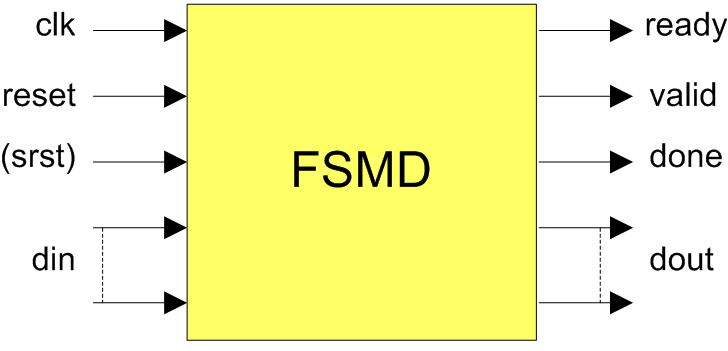
\includegraphics[scale=0.320000]{fsmd-interface.png}}
\caption{FSMD I/O interface.}
\end{figure}

Multi-dimensional data ports are feasible based on their equivalent single-
dimensional flattened array type definition. Then, port selection is a matter of
bitfield extraction. For instance, data input \texttt{din} is defined as
\texttt{din: in std\_logic\_vector(M*N-1 downto 0);}, where \texttt{M},``N`` are generics.
The flattened vector defines \texttt{M} input ports of width \texttt{N}. A selection of
the form \texttt{din((i+1)*N-1 downto i*N)} is typical for a \texttt{for-generate} loop in
order to synthesize iterative structures.

The following example illustrates an element-wise copy of array \texttt{b} to \texttt{c}
without the use of a local array resource. Each interface array consists of 10
elements. It should be assumed that the physical content of both arrays lies in
distributed LUT RAM, from which custom connections can be implemented.

Fig. \hyperref[fsmd-arrif-nac]{fsmd-arrif-nac} illustrates the corresponding function \texttt{func1}.
The VHDL interface of \texttt{func1} is shown in Fig. \hyperref[fsmd-arrif-vhdl]{fsmd-arrif-vhdl} where the
the derived array types \texttt{b\_type} and \texttt{c\_type} are used for \texttt{b, c},
respectively. The definitions of these types can be easily devised as aliases
to a basic type denoted as:
\texttt{type cdt\_type is array (9 downto 0) of std\_logic\_vector(31 downto 0);}.
Then, the alias for \texttt{b} is: \texttt{alias b\_type is cdt\_type;}

\phantomsection\label{fsmd-arrif-nac}
Array-to-array copy without intermediate storage (NAC).
%
\begin{quote}{\ttfamily \raggedright \noindent
procedure~func1~(in~s32~b{[}10{]},\\
~~~~~~~~~~~~~~~~~out~s32~c{[}10{]})~\{\\
~~localvar~s32~i,~t;\\
S\_1:\\
~~i~<=~ldc~0;\\
~~S\_2~<=~jmpun;\\
S\_2:\\
~~S\_3,~S\_EXIT~<=~jmplt~i,~10;\\
S\_3:\\
~~t~<=~load~b,~i;\\
~~c~<=~store~t,~i;\\
~~i~<=~add~i,~1;\\
~~S\_2~<=~jmpun;\\
S\_EXIT:\\
~~nop;\\
\}
}
\end{quote}

\phantomsection\label{fsmd-arrif-vhdl}
Array-to-array copy without intermediate storage (VHDL interface).
%
\begin{quote}{\ttfamily \raggedright \noindent
entity~func1~is\\
~~port~(\\
~~~~clk~~~:~in~~std\_logic;\\
~~~~reset~:~in~~std\_logic;\\
~~~~start~:~in~~std\_logic;\\
~~~~b~~~~~:~in~~b\_type;\\
~~~~c~~~~~:~out~c\_type;\\
~~~~done~~:~out~std\_logic;\\
~~~~ready~:~out~std\_logic\\
~~);\\
end~func1;
}
\end{quote}


\subsection{7.2~~~Architecture and organization%
  \label{architecture-and-organization}%
}

The FSMDs are organized as computations allocated into n+2 states, where n is
the number of required control steps as derived by an operation scheduler. The
two overhead states are the entry (\texttt{S\_ENTRY}) and the exit (\texttt{S\_EXIT}) states
which correspond to the source and sink nodes of the CDFG of the given
procedure, respectively.

Fig. \hyperref[fsmd-minimal]{fsmd-minimal} shows the absolute minimal example of a compliant FSMD
written in VHDL. The FSMD is described in a two-process style using one process
for the current state logic and another process for a combined description of
the next state and output logic. This code will serve as a running example for
better explaining the basic concepts of the FSMD paradigm.

The example of Fig. \hyperref[fsmd-minimal-vhdl]{fsmd-minimal-vhdl} implements the computation of assigning
a constant value to the output port of the FSMD: \texttt{outp <= ldc 42;}. Thus,
lines 5-{}-14 declare the interface (entity) for the hardware block, assuming that
\texttt{outp} is a 16-bit quantity. The FSMD requires three states. In line 17, a
state type enumeration is defined consisting of types \texttt{S\_ENTRY, S\_EXIT} and
\texttt{S\_1}. Line 18 defines the signal 2-tuple for maintaining the state register,
while in lines 19-{}-20 the output register is defined. The current state logic
(lines 25-{}-34) performs asynchonous reset to all storage resources and assigns
new contents to both the state and output registers. Next state and output logic
(lines 37-{}-57) decode \texttt{current\_state} in order to determine the necessary
actions for the computational states of the FSMD. State \texttt{S\_ENTRY} is the idle
state of the FSMD. When the FSMD is driven to this state, it is assumed ready to
accept new input, thus the corresponding status output is raised. When a start
prompt is given externally, the FSMD is activated and in the next cycle, state
\texttt{S\_1} is reached. In \texttt{S\_1} the action of assigning \texttt{CNST\_42} to \texttt{outp}
is performed. Finally, when state \texttt{S\_EXIT} is reached, the FSMD declares the
end of all computations via \texttt{done} and returns to its idle state.

It should be noted that this design approach is a rather conservative one. One
possible optimization that can occur in certain cases is the merging of
computational states that immediately prediate the sink state (\texttt{S\_EXIT}) with
it.

Fig. \hyperref[fsmd-minimal-timediag]{fsmd-minimal-timediag} shows the timing diagram for the \texttt{minimal} design.
As expected, the overall latency for computing a sample is three machine cycles.

\phantomsection\label{fsmd-minimal}
Minimal FSMD implementation.

\phantomsection\label{fsmd-minimal-vhdl}
Minimal FSMD implementation in VHDL.
%
\begin{quote}{\ttfamily \raggedright \noindent
library~IEEE;\\
use~IEEE.std\_logic\_1164.all;\\
use~IEEE.numeric\_std.all;\\
~\\
entity~minimal~is\\
~~port~(\\
~~~~clk~~~:~in~~std\_logic;\\
~~~~reset~:~in~~std\_logic;\\
~~~~start~:~in~~std\_logic;\\
~~~~outp~~:~out~std\_logic\_vector(15~downto~0);\\
~~~~done~~:~out~std\_logic;\\
~~~~ready~:~out~std\_logic\\
~~);\\
end~minimal;\\
~\\
architecture~fsmd~of~minimal~is\\
~~type~state\_type~is~(S\_ENTRY,~S\_EXIT,~S\_1);\\
~~signal~current\_state,~next\_state:~state\_type;\\
~~signal~outp\_next:~std\_logic\_vector(15~downto~0);\\
~~signal~outp\_reg:~std\_logic\_vector(15~downto~0);\\
~~constant~CNST\_42:~std\_logic\_vector(15~downto~0)~:=\\
~~~~"0000000000101010";\\
begin\\
~~-{}-~current~state~logic\\
~~process~(clk,~reset)\\
~~begin\\
~~~~if~(reset~=~'1')~then\\
~~~~~~current\_state~<=~S\_ENTRY;\\
~~~~~~outp\_reg~<=~(others~=>~'0');\\
~~~~elsif~(clk~=~'1'~and~clk'EVENT)~then\\
~~~~~~current\_state~<=~next\_state;\\
~~~~~~outp\_reg~<=~outp\_next;\\
~~~~end~if;\\
~~end~process;\\
~\\
~~-{}-~next~state~and~output~logic\\
~~process~(current\_state,~start,~outp\_reg)\\
~~begin\\
~~~~done~<=~'0';\\
~~~~ready~<=~'0';\\
~~~~outp\_next~<=~outp\_reg;\\
~~~~case~current\_state~is\\
~~~~when~S\_ENTRY~=>\\
~~~~~~ready~<=~'1';\\
~~~~~~if~(start~=~'1')~then\\
~~~~~~~~next\_state~<=~S\_1;\\
~~~~~~else\\
~~~~~~~~next\_state~<=~S\_ENTRY;\\
~~~~~~end~if;\\
~~~~~~when~S\_1~=>\\
~~~~~~~~outp\_next~<=~CNST\_42;\\
~~~~~~~~next\_state~<=~S\_EXIT;\\
~~~~~~when~S\_EXIT~=>\\
~~~~~~~~done~<=~'1';\\
~~~~~~~~next\_state~<=~S\_ENTRY;\\
~~~~end~case;\\
~~end~process;\\
~~outp~<=~outp\_reg;\\
end~fsmd;
}
\end{quote}
\begin{figure}
\phantomsection\label{fsmd-minimal-timediag}
\noindent\makebox[\textwidth][c]{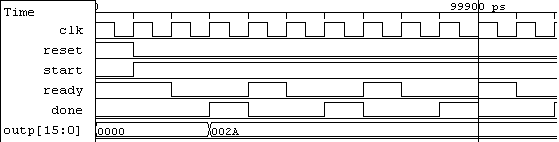
\includegraphics[scale=0.500000]{minimal-timediag.png}}
\caption{Timing diagram for the minimal FSMD.}
\end{figure}

In certain cases, input registering might be desired. This intent can be made
explicit by copying input port data to an internal register. For the case of the
\emph{eda} algorithm, a new localvar, \texttt{a} would be introduced to perform the copy
as \texttt{a <= mov in1;}. The VHDL counterpart is given as \texttt{a\_1\_next <= in1;},
making this data available through register \texttt{a\_1\_reg} in the following cycle.
For register \texttt{r}, signal \texttt{r\_next} represents the value that is available at
the register input, and \texttt{r\_reg} the stored data in the register.


\subsubsection{7.2.1~~~Communication with embedded memories%
  \label{communication-with-embedded-memories}%
}

Array objects can be synthesized to block RAMs in contemporary FPGAs. These
embedded memories support fully synchronous read and write operations. A
requirement for asynchronous read mandates the use of memory residing in
distributed LUT storage.

In BASIL, the \texttt{load} and \texttt{store} primitives are used for describing read and
write memory access. We will assume a RAM memory model with write enable, and
separate data input (\texttt{din}) and output (\texttt{dout}) sharing a common address
port (\texttt{rwaddr}). To control access to such block, a set of four non-trivial
signals is needed: \texttt{mem\_we}, a write enable signal, and the corresponding
signals for addressing, data input and output.

\texttt{store} is the simpler operation of the two. It requires raising \texttt{mem\_we}
in a given single-cycle state so that data are stored in memory and made
available in the subsequent state/machine cycle.

Synchronous \texttt{load} requires the introduction of a \texttt{waitstate} register.
This register assists in devising a dual-cycle state for performing the load.
Fig. \hyperref[fsmd-loadstore-vhdl]{fsmd-loadstore-vhdl} illustrates the implementation of a load operation.
During the first cycle of \texttt{STATE\_1} the memory block is addressed. In the
second cycle, the requested data are made available through \texttt{mem\_dout} and
are assigned to register \texttt{mysignal}. This data can be read from
\texttt{mysignal\_reg} during \texttt{STATE\_2}.

\phantomsection\label{fsmd-loadstore-vhdl}
Wait-state-based communication for loading data from a block RAM.
%
\begin{quote}{\ttfamily \raggedright \noindent
when~STATE\_1~=>\\
~~mem\_addr~<=~index;\\
~~waitstate\_next~<=~not~(waitstate\_reg);\\
~~if~(waitstate\_reg~=~'1')~then\\
~~~~mysignal\_next~<=~mem\_dout;\\
~~~~next\_state~<=~STATE\_2;\\
~~else\\
~~~~next\_state~<=~STATE\_1;\\
~~end~if;\\
when~STATE\_2~=>\\
~~...
}
\end{quote}


\subsubsection{7.2.2~~~Hierarchical FSMDs%
  \label{hierarchical-fsmds}%
}

Our extended FSMD concept allows for hierarchical FSMDs defining entire systems
with calling and callee CDFGs. A two-state protocol can be used to describe
a proper communication between such FSMDs. The first state is considered
as the \emph{preparation} state for the communication, while the latter state
actually comprises an \emph{evaluation} superstate where the entire computation
applied by the callee FSMD is effectively hidden.

The calling FSMD performs computations where new values are assigned
to \texttt{*\_next} signals and registered values are read from \texttt{*\_reg} signals. To
avoid the problem of multiple signal drivers, callee procedure instances produce
\texttt{*\_eval} data outputs that can then be connected to register inputs by
hardwiring to the \texttt{*\_next} signal.

Fig. \hyperref[fsmd-pcall-vhdl]{fsmd-pcall-vhdl} illustrates a procedure call to an integer square root
evaluation procedure. This procedure uses one input and one output
\texttt{std\_logic\_vector} operands, both considered to represent integer values.
Thus, a procedure call of the form \texttt{(m) <= isqrt(x);} is implemented by
the given code segment.

\phantomsection\label{fsmd-pcall-vhdl}
State-superstate-based communication of a caller and callee procedure instance
in VHDL.
%
\begin{quote}{\ttfamily \raggedright \noindent
when~STATE\_1~=>\\
~~isqrt\_start~<=~'1';\\
~~next\_state~<=~SUPERSTATE\_2;\\
when~SUPERSTATE\_2~=>\\
~~if~((isqrt\_ready~=~'1')~and~(isqrt\_start~=~'0'))~then\\
~~~~m\_next~<=~m\_eval;\\
~~~~next\_state~<=~STATE\_3;\\
~~else\\
~~~~next\_state~<=~SUPERSTATE\_2;\\
~~end~if;\\
when~STATE\_3~=>\\
...\\
isqrt\_0~:~entity~WORK.isqrt(fsmd)\\
~~port~map~(\\
~~~~clk,~reset,\\
~~~~isqrt\_start,~x\_reg,~m\_eval,\\
~~~~isqrt\_done,~isqrt\_ready\\
~~);
}
\end{quote}

\texttt{STATE\_1} sets up the callee instance. The following state is a superstate
where control is transferred to the component instance of the callee. When
the callee instance terminates its computation, the \texttt{ready} signal is raised.
Since the \texttt{start} signal of the callee is kept low, the generated output data
can be transferred to the \emph{m} register via its \texttt{m\_next} input port. Control
then is handed over to state \texttt{STATE\_3}.

The callee instance follows the established FSMD interface, reading \texttt{x\_reg}
data and producing an exact integer square root in \texttt{m\_eval}. Multiple copies
of a given callee are supported by versioning of the component instances.


\subsubsection{7.2.3~~~Steaming ports%
  \label{steaming-ports}%
}

ANSI C is the archetypical example of a general-purpose imperative language that
does not support streaming primitives, i.e. it is not possible for someone to
express and process streams solely based on the semantics of such language.

Streaming suits applications with absence of control flow. In a prime
factorization algorithm (\emph{pfactor}), a streaming output can be used, \texttt{outp},
to produce successive factors. The streaming port is accessed based on
\texttt{valid}. Thus, \texttt{outp} is accessed periodically in context of basic block
\texttt{BB4} as shown in \hyperref[fsmd-pfactor-nac]{fsmd-pfactor-nac}.

\phantomsection\label{fsmd-pfactor-nac}
NAC code for a prime factorization algorithm involving output streaming.
%
\begin{quote}{\ttfamily \raggedright \noindent
procedure~pfactor~(in~u16~x,~out~u16~outp)~\{\\
~~localvar~u16~i,~n,~t0;\\
BB1:\\
~~n~<=~mov~x;\\
~~i~<=~ldc~2;\\
~~BB2~<=~jmpun;\\
BB2:\\
~~BB3,~BB\_EXIT~<=~jmple~i,~n;\\
BB3:\\
~~t0~<=~rem~n,~i;\\
~~BB4,~BB5~<=~jmpeq~t0,~0;\\
BB4:\\
~~n~<=~div~n,~i;\\
~~outp~<=~mov~i;\\
~~BB3~<=~jmpun;\\
BB5:\\
~~i~<=~add~i,~1;\\
~~BB2~<=~jmpun;\\
BB\_EXIT:\\
~~nop;\\
\}
}
\end{quote}


\subsubsection{7.2.4~~~Operation chaining%
  \label{operation-chaining}%
}

Operation chaining assigns dependent SSA operations to a single control step.
Simple means for selective operation chaining involve merging successive ASAP
states. In successive states, intermediate registers are eliminated by wiring
assignments to \texttt{*\_next} signals and reusing them in the subsequent chained
computation, instead of reading from the stored \texttt{*\_reg} value. To avoid
excessive critical paths, a heuristic is defined for disallowing flow-dependent
multiple occurrences of expensive operators in the same newly defined state.

In Fig. \hyperref[fsmd-eda-chaining]{fsmd-eda-chaining} states \texttt{S\_1\_3} to \texttt{S\_1\_5} comprise intermediate
computations in a merged \texttt{S\_1\_1} state.

\phantomsection\label{fsmd-eda-nochaining}
2D euclidean distance approximation algorithm (\emph{eda}) without chained
computations.
%
\begin{quote}{\ttfamily \raggedright \noindent
...\\
when~S\_1\_3~=>\\
~~t3\_next~<=~"000"\&x\_reg(15~downto~3);\\
~~t4\_next~<=~"0"\&y\_reg(15~downto~1);\\
~~next\_state~<=~S\_1\_4;\\
when~S\_1\_4~=>\\
~~t5\_next~<=~x\_reg~-~t3\_reg;\\
~~next\_state~<=~S\_1\_5;\\
when~S\_1\_5~=>\\
~~t6\_next~<=~t4\_reg~+~t5\_reg;\\
~~next\_state~<=~S\_1\_6;
}
\end{quote}

\phantomsection\label{fsmd-eda-chaining}
2D euclidean distance approximation algorithm (\emph{eda}) with chained computations.
%
\begin{quote}{\ttfamily \raggedright \noindent
when~S\_1\_1~=>\\
~~...\\
~~t3\_next~<=~"000"\&x\_next(15~downto~3);\\
~~t4\_next~<=~"0"\&y\_next(15~downto~1);\\
~~t5\_next~<=~x\_next~-~t3\_next;\\
~~t6\_next~<=~t4\_next~+~t5\_next;\\
~~...
}
\end{quote}


\section{8~~~The HercuLeS GUI%
  \label{the-hercules-gui}%
}


\subsection{8.1~~~Introduction%
  \label{id3}%
}

The \href{http://www.ajaxcompilers.com/technology/hercules-high-level-synthesis}{HercuLeS} 1.0 (2013a) distribution includes a graphical user interface (GUI) for allowing user-friendly access to HercuLeS HLS without the burden of coping with command-line syntax. The main purpose of the GUI is for the user to control code generation, simulation and synthesis options via an intuitive scheme. The user
sets various options for the overall process from within the GUI (by interacting with checkbuttons, radiobuttons, entries, text widgets etc) in order for a shell script to be generated which will steer these tasks transparently. For running the generated script, a minimal Unix bash script environment is expected. On Windows, the \href{http://www.mingw.org}{MinGW} and msys distributions are suggested. On Linux, the required facilities are natively supported in almost any distributions, including Ubuntu Linux 12.04 LTS.

To summarize, the HercuLeS GUI performs the following tasks:
%
\begin{itemize}

\item Allow the user to set various options and to load a C or NAC program file for processing

\item Optionally, load a configuration file (which automatically sets all necessary options)

\item Generate the HercuLeS run script

\item Execute the HercuLeS run script

\item View results from within an included results browser.

\end{itemize}

The HercuLeS GUI can be accessed by double-clicking on the icon of the \texttt{hercules.exe} executable, or by command-line invocation as follows:

\begin{DUlineblock}{0em}
\item[] \DUroletitlereference{./gui/hercules.exe}
\end{DUlineblock}

from within the top-level directory of your HercuLeS installation.

The HercuLeS GUI executable is available on both 32-bit Windows and 32-bit Linux.


\subsection{8.2~~~Overview%
  \label{id4}%
}

When executing \texttt{hercules.exe}, a splashscreen appears for a few seconds, as shown in Fig. \hyperref[hercules-gui-splashscreen]{hercules-gui-splashscreen}.
\begin{figure}
\phantomsection\label{hercules-gui-splashscreen}
\noindent\makebox[\textwidth][c]{
\includegraphics[scale=0.400000]{hercules-gui-splashscreen.png}}
\caption{The HercuLeS GUI splashscreen.}
\end{figure}

After the lapse of a few seconds, the basic configuration screen of HercuLeS is visible. A nominal view of the GUI is shown in Fig. \hyperref[hercules-gui-basicscreen]{hercules-gui-basicscreen}.
The GUI consists of the following:
%
\begin{itemize}

\item a dropdown menu with the \texttt{File}, \texttt{General}, \texttt{Action}, \texttt{Configuration}, \texttt{Theme} (on the left side) and \texttt{Help} (on the right side) submenus.

\item A set of basic framed controls for setting the simulator (\texttt{Simulator}), waveform generation settings (\texttt{Output waveform format}), simulation and synthesis options (\texttt{Simulation and synthesis options}) and miscellaneous options (\texttt{Miscellaneous options}).

\item A notebook for controlling high-level synthesis settings in detail, which consists of four tabs: \texttt{General}, \texttt{Optimizations}, \texttt{Operation scheduling} and \texttt{Code generation}.

\item The read-only console where the standard output is logged in real-time in order to examine the progress of the current run.

\item A set of buttons: \texttt{Run HercuLeS}, \texttt{Results browser}, \texttt{Clear generated files}, \texttt{Clear console} (on the left), and \texttt{Exit} (on the right). Except \texttt{Run HercuLeS}, all other buttons are disabled at startup.

\end{itemize}
\begin{figure}
\phantomsection\label{hercules-gui-basicscreen}
\noindent\makebox[\textwidth][c]{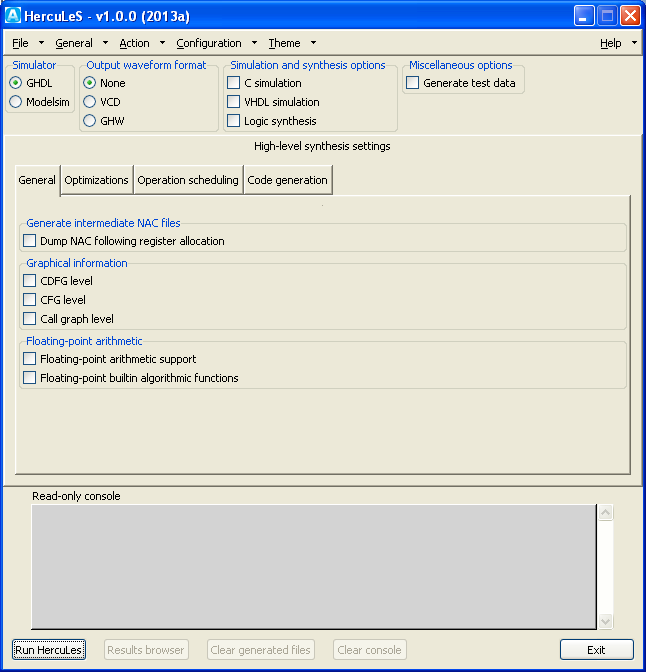
\includegraphics[scale=0.400000]{hercules-gui-basicscreen.png}}
\caption{The initial HercuLeS GUI screen immediately after invocation.}
\end{figure}

A major element of the HercuLeS GUI which is not readily visible is the \texttt{Results browser}. This element is activated after a successful run of generating and executing a HercuLeS run script for a specific C or NAC translation unit.

It should be noted that context-specific balloon help is available for most visible controls. This kind of help of accessible simply by mouse hovering over the corresponding GUI element.


\subsection{8.3~~~Quick-start guide%
  \label{quick-start-guide}%
}

The fastest and simplest way to use the HercuLeS GUI is a four-step process. Using this process, the user is able to perform C simulation, VHDL simulation and logic synthesis on the generated C and VHDL representation of a specified C or NAC program file.

The process is as follows:
\setcounter{listcnt0}{0}
\begin{list}{\arabic{listcnt0}.}
{
\usecounter{listcnt0}
\setlength{\rightmargin}{\leftmargin}
}

\item From the \texttt{File} menu either load a C application (\texttt{Load C program file}) or a NAC application (\texttt{Load NAC program file}).

\item From the \texttt{File} menu, press \texttt{Load HercuLeS configuration} and choose \texttt{default.config}.

\item From the \texttt{Action} menu, press \texttt{Run HercuLeS} (or press the always visible \texttt{Run HercuLeS} button near the bottom-left corner of the basic screen layout.

\item When enabled, press \texttt{Results browser} from the bottom-left corner of the basic screen layout. This will invoke the results browser.
\end{list}

Fig. \hyperref[hercules-gui-quickstart]{hercules-gui-quickstart} depicts graphically the proposed four-step process for quickly setting up and processing a program file with HercuLeS.
\begin{figure}
\phantomsection\label{hercules-gui-quickstart}
\noindent\makebox[\textwidth][c]{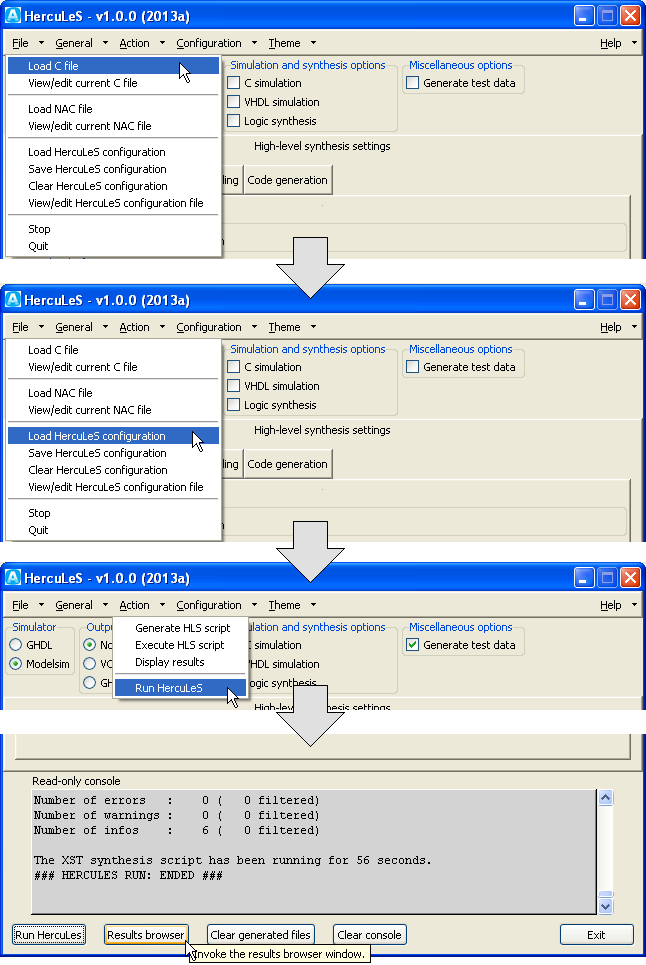
\includegraphics[scale=0.400000]{hercules-gui-quickstart.png}}
\caption{The four-step quick-start process for using the HercuLeS GUI.}
\end{figure}


\subsection{8.4~~~The GUI in detail%
  \label{the-gui-in-detail}%
}


\subsubsection{8.4.1~~~Dropdown menus%
  \label{dropdown-menus}%
}


\paragraph{8.4.1.1~~~File submenu%
  \label{file-submenu}%
}

From left to right, the first dropdown menu is \texttt{File} which covers basic file opening/loading, viewing and editing operations. It is shown in Fig. \hyperref[hercules-gui-ddmenu-file]{hercules-gui-ddmenu-file}.
\begin{figure}
\phantomsection\label{hercules-gui-ddmenu-file}
\noindent\makebox[\textwidth][c]{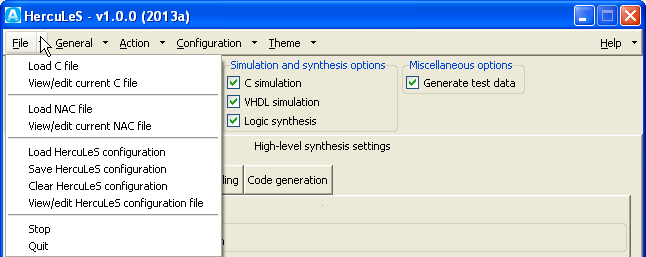
\includegraphics[scale=0.400000]{hercules-gui-ddmenu-file.png}}
\caption{Dropdown menu for file loading, viewing and editing.}
\end{figure}

HercuLeS can process either C or NAC single-translation-unit programs. The first set of options deal with handling C program files. \texttt{Load C file} allows for loading a C file for processing with a \texttt{.c} extension. To view and optionally edit the file, the selection \texttt{View/edit current C file} is used. To view or edit a C file, the C file should be already loaded, otherwise a relevant popup message box will appear to prompt for loading a C file.

The builtin editor/viewer for C files (the same goes for NAC and configuration files) allows to save your changes but not to rename the loaded file. Fig. \hyperref[hercules-gui-fileviewer]{hercules-gui-fileviewer} shows a C program file in the file editor/viewer.
\begin{figure}
\phantomsection\label{hercules-gui-fileviewer}
\noindent\makebox[\textwidth][c]{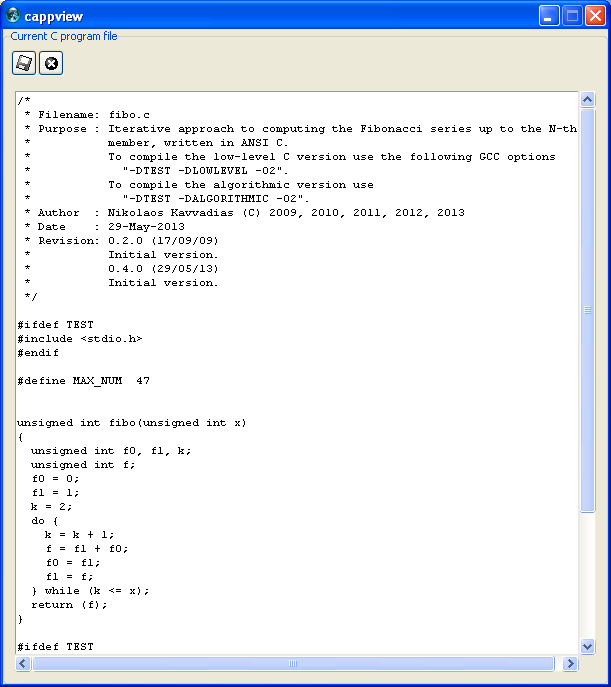
\includegraphics[scale=0.400000]{hercules-gui-fileviewer.png}}
\caption{C file editor/viewer in the HercuLeS GUI.}
\end{figure}

In order to load NAC files, \texttt{Load NAC file} is used. NAC files are expected to have either an \texttt{.nac}, \texttt{.asm}, or \texttt{.s} extensions, since NAC (N-Address Code) programs are essentially written in a form of typed-assembly language. Upon selection, the corresponding NAC file is automatically loaded for processing.To view and optionally edit the file, the selection \texttt{View/edit current NAC file} is used. To view or edit a NAC file, the NAC file should be already loaded, otherwise a relevant popup message box will appear to prompt for loading a NAC file.

The builtin editor/viewer for NAC files is similar to the one used for editing and viewing ANSI/ISO C program files.

HercuLeS configuration files allow the user to supply a full set of configuration options to HercuLeS without interfering with the GUI elements. As a result, loading a translation unit for processing and configuring HercuLeS has a much smaller turnaround time. Configuration files have the \texttt{.config} suffix; their format is explained in the corresponding section. The option \texttt{Load HercuLeS configuration} allows for loading a configuration file. The HercuLeS distribution comes with at least one predefined configuration file, named \texttt{default.config}.

Configuration files can be saved under different names. This is a useful feature for the user, and enables the backup and storage of an existing configuration, e.g. one setup interactively by the user. \texttt{Save HercuLeS configuration} popups the corresponding dialog for storing the current configuration as a configuration file.

To clear the loaded configuration, \texttt{Clear HercuLeS configuration} is used. The result is that only minimal settings will be loaded, for instance no HDL simulation and logic synthesis will be enabled on this setting.

To view and optionally edit the configuration file, the selection \texttt{View/edit HercuLeS configuration file} is used. To view or edit a configuration file, the configuration file should be already loaded, otherwise a relevant popup message box will appear to prompt for loading a configuration file.

The options \texttt{Stop} and \texttt{Quit} allow for ending the current run of HercuLeS abruptly, and to exit the environment, correspondingly. These options are equivalent to pressing \texttt{<Control-C>} and \texttt{<Control-Q>} from the keyboard during a HercuLeS session.


\paragraph{8.4.1.2~~~General submenu%
  \label{general-submenu}%
}

The second dropdown menu is \texttt{General} which is a placeholder for options that can be applied in general to all tools that are invoked by HercuLeS. Specifically, the \texttt{nac2cdfg} translator from NAC to Graphviz CDFGs and the \texttt{cdfg2hdl} backend (HDL code generator from \href{http://www.graphviz.org}{Graphviz} CDFGs) are affected by the options of this dropdown menu.
This menu is shown in Fig. \hyperref[hercules-gui-ddmenu-general]{hercules-gui-ddmenu-general}.
\begin{figure}
\phantomsection\label{hercules-gui-ddmenu-general}
\noindent\makebox[\textwidth][c]{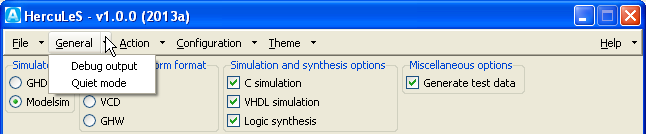
\includegraphics[scale=0.400000]{hercules-gui-ddmenu-general.png}}
\caption{Dropdown menu for general options.}
\end{figure}

\texttt{Debug output} enables the emission of additional diagnostic information to the standard output during a HercuLeS script run. This includes printouts of the contents of various internal data structures of both \texttt{nac2cdfg} and \texttt{cdfg2hdl}.

\texttt{Quiet mode} disables the emission to the standard output of both any additional diagnostic information as well as other informative messages during a HercuLeS script run. When enabling this mode, only indications of the start and end of a HercuLeS script run are generated and depicted in the read-only console.


\paragraph{8.4.1.3~~~Action submenu%
  \label{action-submenu}%
}

The third dropdown menu is \texttt{Action} which provides several controls for generating and executing a HercuLeS run script, as well as displaying the generated result files in a custom browser, optimized for this purpose.

Fig. \hyperref[hercules-gui-ddmenu-action]{hercules-gui-ddmenu-action} illustrates the corresponding submenu.
\begin{figure}
\phantomsection\label{hercules-gui-ddmenu-action}
\noindent\makebox[\textwidth][c]{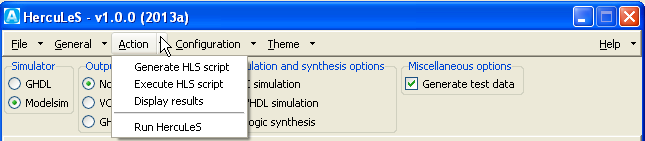
\includegraphics[scale=0.400000]{hercules-gui-ddmenu-action.png}}
\caption{Dropdown menu for script action options.}
\end{figure}

\texttt{Generate HLS script} should be used when the user has already setup either a C or NAC program file and has loaded or interactively specified a configuration. By clicking this menubutton, the HercuLeS script for the specified application is generated. The generated script is a bash shell script which follows the naminb convention \texttt{hercules-app.sh}, where \texttt{app} is the name of the C or NAC program file. \texttt{app} should be the same to the name of the top-level procedure in the specified translation unit.

\texttt{Execute HLS script} can be used for forcing the execution of the generated HercuLeS run script. All actions that are performed by the HercuLeS run script (or HLS script) are logged in real-time to the read-only console. Script execution start is indicated by the following message:

\begin{DUlineblock}{0em}
\item[] \texttt{\#\#\# HERCULES RUN: STARTED \#\#\#}
\end{DUlineblock}

while when script execution completes, the following message is generated to wrap up the contents of standard output:

\begin{DUlineblock}{0em}
\item[] \texttt{\#\#\# HERCULES RUN: ENDED \#\#\#}
\end{DUlineblock}

Following the completion of HercuLeS run script execution, \texttt{Display results} can be used to load the results browser. The results browser provides a tree-view of each generated item (file) and allows for easy viewing of the contents of this file, when applicable in graphical form.

The \texttt{Run HercuLeS} menubutton when selected applies all the three previous actions in sequence:
%
\begin{itemize}

\item Generate HLS script

\item Execute HLS script

\item Display results

\end{itemize}

No further user intervention is required for generating the script for driving the high-level synthesis process, executing the script, invoking all necessary external tools (such as the host C compiler, HDL simulators and the \href{http://www.xilinx.com}{Xilinx} ISE/XST logic synthesis tool), and loading the results browser when HLS has completed.


\paragraph{8.4.1.4~~~Configuration submenu%
  \label{configuration-submenu}%
}

The fourth dropdown menu is \texttt{Configuration} which provides layouts with entries and choices for configuring external tools and to provide information on the host system setup.

Fig. \hyperref[hercules-gui-ddmenu-config]{hercules-gui-ddmenu-config} illustrates the corresponding submenu.
\begin{figure}
\phantomsection\label{hercules-gui-ddmenu-config}
\noindent\makebox[\textwidth][c]{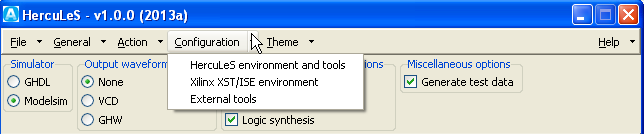
\includegraphics[scale=0.400000]{hercules-gui-ddmenu-config.png}}
\caption{Dropdown menu for environment and external tool configuration options.}
\end{figure}

\texttt{HercuLeS environment and tools} provides access to \texttt{Environment configuration} options for the HercuLeS setup (HercuLeS installation path), host compiler options, HercuLeS frontend options and source optimizer options. Fig. \hyperref[hercules-gui-ddmenu-config-env]{hercules-gui-ddmenu-config-env} shows the default environment configuration options.
\begin{figure}
\phantomsection\label{hercules-gui-ddmenu-config-env}
\noindent\makebox[\textwidth][c]{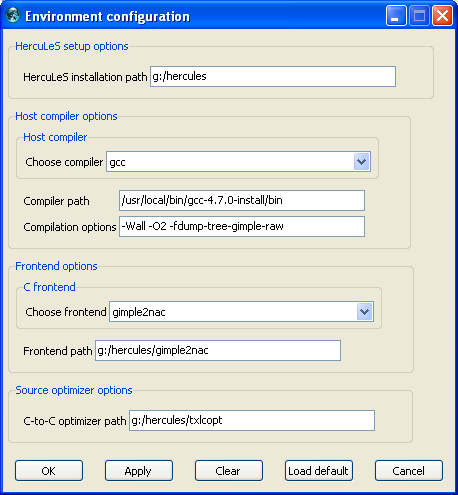
\includegraphics[scale=0.400000]{hercules-gui-ddmenu-config-env.png}}
\caption{Layout for specifying environment configuration options.}
\end{figure}

As the host compiler, either \texttt{gcc} or \texttt{llvm} can be used. This choice affects the host compiler (either \href{http://gcc.gnu.org}{GCC} or \href{http://llvm.org}{LLVM}) used for test data generation and backend C code simulation. Within the same set of options, the path to the \texttt{/bin} directory of the host compiler can be set (currently this is left unused; the host compiler is assumed to be in the system \texttt{PATH} environmental variable). Further, a string specifying the compilation options passed to the host compiler is specified in \texttt{Compilation options}, however this is only used with the \texttt{gimple2nac} HercuLeS frontend, since it affects only this case.

\texttt{Frontend options} provide a choice among to distinct ANSI C frontends, \texttt{gimple2nac} which uses GIMPLE intermediate dumps generated by \texttt{gcc} in order to extract the corresponding NAC representation of the application, and \texttt{irc2nac} which uses a custom translator from IR-C (a low-level C subset, generated by a port of the LANCE compiler) to NAC. The \texttt{Frontend path} entry should direct to the directory where the executable of the corresponding frontend is placed.

\texttt{Source optimizer options} specifies the top-level directory of the included C-to-C source optimizer provided with the HercuLeS distribution. This optimizer is named \texttt{txlcopt} and is nominally placed in the \texttt{/txlcopt} subdirectory of the HercuLeS distribution.

At the bottom of the \texttt{Environment configuration} layout, several buttons are located. The \texttt{OK} button is used to close this dialog without further changes. \texttt{Apply} stores the current settings of the environment configuration. \texttt{Clear} removes all user-specified settings. \texttt{Load default} reinstantiates the predefined defaults which are specified in the \texttt{hercules.ini} initialization file. \texttt{Cancel} allows to cancel the current operation.

This five-button configuration is used for all configuration layouts that are accessible through the \texttt{Configuration} dropdown menu.

\texttt{Xilinx XST/ISE environment} provides access to \texttt{Xilinx XST/ISE configuration} options for the the Xilinx XST/ISE external logic synthesis tool. Fig. \hyperref[hercules-gui-ddmenu-config-xst]{hercules-gui-ddmenu-config-xst} shows the default Xilinx XST/ISE configuration options.
\begin{figure}
\phantomsection\label{hercules-gui-ddmenu-config-xst}
\noindent\makebox[\textwidth][c]{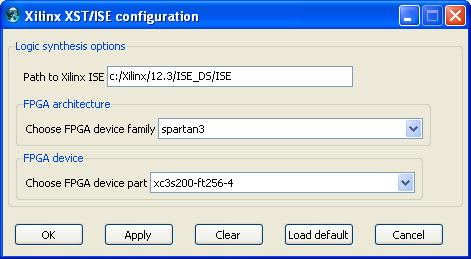
\includegraphics[scale=0.400000]{hercules-gui-ddmenu-config-xst.png}}
\caption{Layout for specifying Xilinx XST/ISE configuration options.}
\end{figure}

\texttt{Path to Xilinx ISE} is an entry for setting the path to the \texttt{ISE} directory of the user's Xilinx ISE/XST installation. A specific FPGA architecture and device should be specified in order to be picked up by the synthesis process. Thus, the user should specify a meaningful combination of an FPGA architecture (\texttt{Choose FPGA device family}) and FPGA device (\texttt{Choose FPGA device part}). The following combinations are the ones that are supported in HercuLeS v1.0.0 (2013a):
%
\begin{itemize}

\item spartan3 with xc3s200-ft256-4

\item virtex4 with xc4vlx25-ff668-10

\item virtex6 with xc6vlx75t-ff484-1

\end{itemize}

The corresponding dropdown widget elements allow for the user to add other choices as well. The dropdown lists can be updated to show all entries by selecting \texttt{Load default}. This issue appears to be as a bug in the \href{http://www.satisoft.com/tcltk/gridplus2/}{GRIDPLUS} widget set which is used for the configuration layouts.

\texttt{External tools} provides access to \texttt{External tools configuration} options for third-party external tools e.g. for image visualization. An example of a default layout for these options is shown in Fig. \hyperref[hercules-gui-ddmenu-config-xtools]{hercules-gui-ddmenu-config-xtools}.
\begin{figure}
\phantomsection\label{hercules-gui-ddmenu-config-xtools}
\noindent\makebox[\textwidth][c]{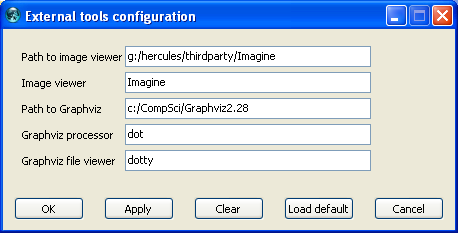
\includegraphics[scale=0.400000]{hercules-gui-ddmenu-config-xtools.png}}
\caption{Layout for specifying third-party tool configuration options.}
\end{figure}

Currently, these options specify the path and name of the image viewer. In addition, the path to the Graphviz distribution (which should be installed in the user's machine) as well as the name of the Graphviz processor (\texttt{dot}) and the preferred Graphviz file viewer (one option is \texttt{dotty}, which is bundled with all Graphviz distributions; other choices are also offered by other third parties).

HercuLeS comes on Windows with a free for-commercial-use image viewer named \href{http://www.nyam.pe.kr/}{Imagine}. The proper local path to \texttt{Imagine} is thus automatically specified. However, the user can bypass this setting by providing the details for the image viewer of preference.


\paragraph{8.4.1.5~~~Theme submenu%
  \label{theme-submenu}%
}

The fifth dropdown menu is \texttt{Theme} which provides simple access to all available themes of the host execution platform. Fig. \hyperref[hercules-gui-ddmenu-theme]{hercules-gui-ddmenu-theme} illustrates the corresponding submenu as it appears in a typical Windows XP installation using \href{http://www.activestate.com/activetcl}{ActiveTcl} 8.5.14.
\begin{figure}
\phantomsection\label{hercules-gui-ddmenu-theme}
\noindent\makebox[\textwidth][c]{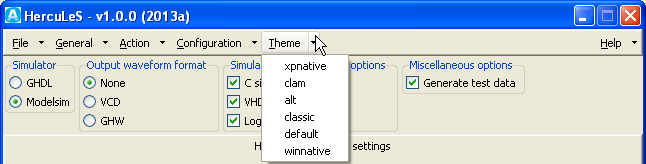
\includegraphics[scale=0.400000]{hercules-gui-ddmenu-theme.png}}
\caption{Dropdown menu for changing the GUI theme.}
\end{figure}

In this example, the following themes are accessible:
%
\begin{itemize}

\item \texttt{xpnative}

\item \texttt{clam}

\item \texttt{alt}

\item \texttt{classic}

\item \texttt{default}

\item \texttt{winnative}.

\end{itemize}

For a Linux installation, the available set of themes could be possibly much different. In all cases, all available themes will be accessible through this dropdown submenu.

The following set of figures illustrate the appearance of the basic GUI screen using the different themes on Windows.
\begin{figure}
\phantomsection\label{hercules-gui-basicscreen-xpnative}
\noindent\makebox[\textwidth][c]{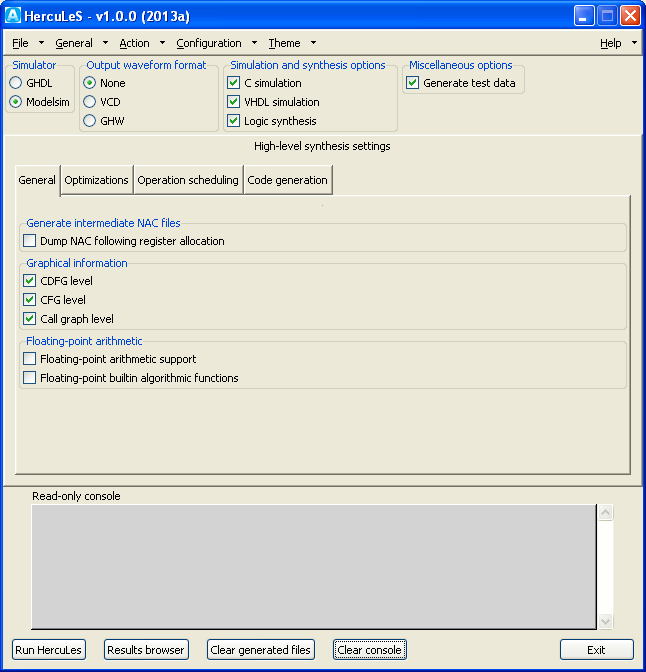
\includegraphics[scale=0.400000]{hercules-gui-basicscreen-xpnative.png}}
\caption{Basic GUI screen using the \texttt{xpnative} theme on Windows.}
\end{figure}
\begin{figure}
\phantomsection\label{hercules-gui-basicscreen-clam}
\noindent\makebox[\textwidth][c]{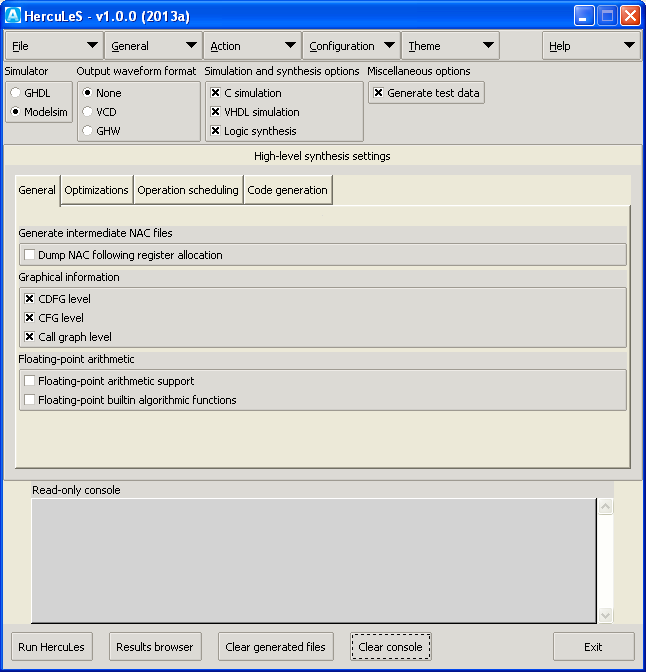
\includegraphics[scale=0.400000]{hercules-gui-basicscreen-clam.png}}
\caption{Basic GUI screen using the \texttt{clam} theme on Windows.}
\end{figure}
\begin{figure}
\phantomsection\label{hercules-gui-basicscreen-alt}
\noindent\makebox[\textwidth][c]{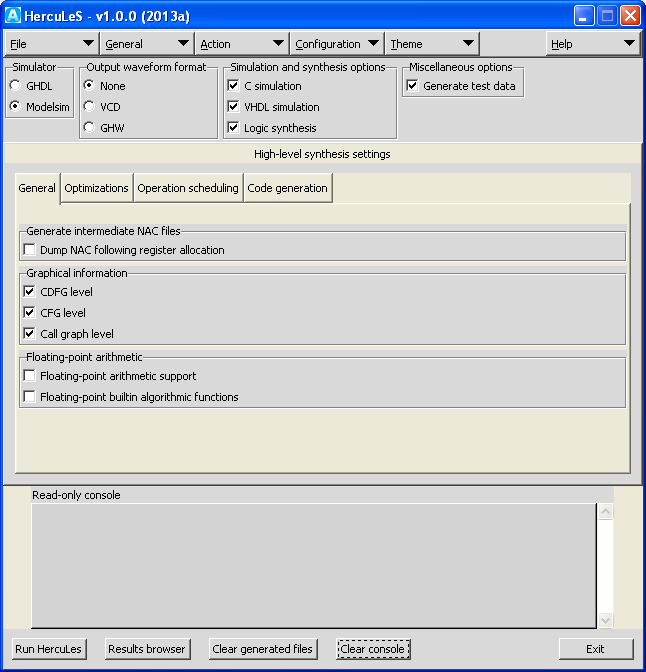
\includegraphics[scale=0.400000]{hercules-gui-basicscreen-alt.png}}
\caption{Basic GUI screen using the \texttt{alt} theme on Windows.}
\end{figure}
\begin{figure}
\phantomsection\label{hercules-gui-basicscreen-classic}
\noindent\makebox[\textwidth][c]{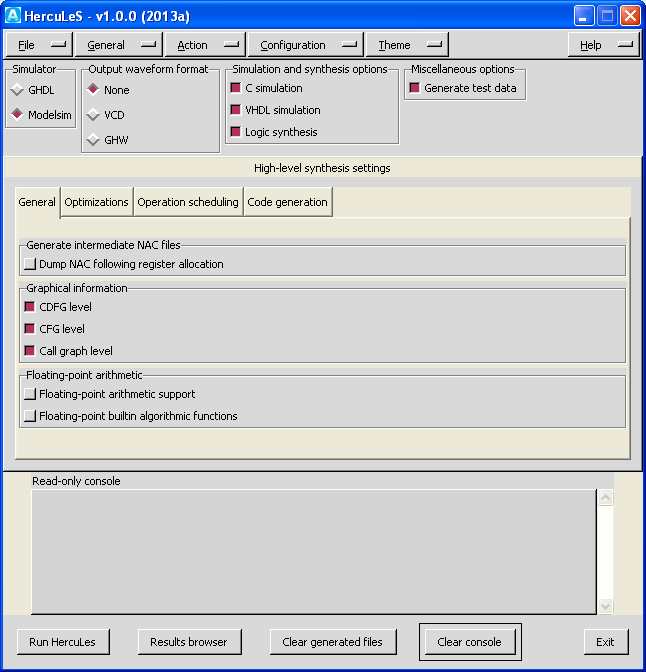
\includegraphics[scale=0.400000]{hercules-gui-basicscreen-classic.png}}
\caption{Basic GUI screen using the \texttt{classic} theme on Windows.}
\end{figure}
\begin{figure}
\phantomsection\label{hercules-gui-basicscreen-default}
\noindent\makebox[\textwidth][c]{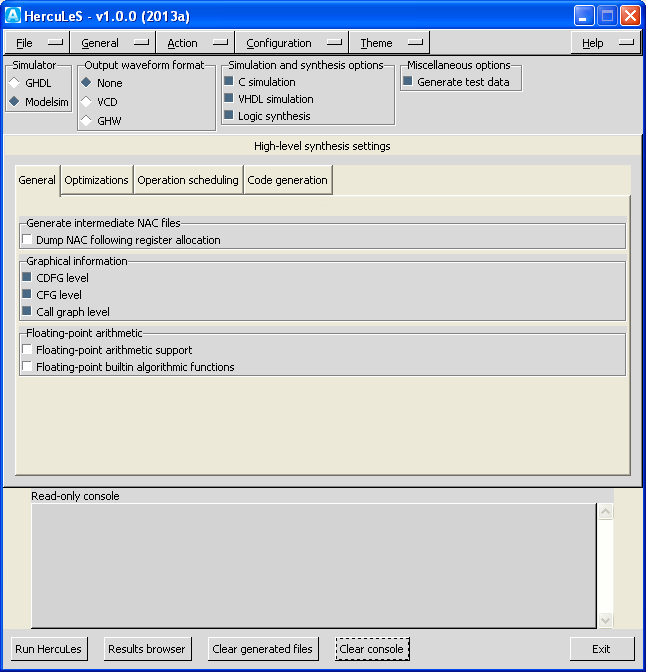
\includegraphics[scale=0.400000]{hercules-gui-basicscreen-default.png}}
\caption{Basic GUI screen using the \texttt{default} theme on Windows.}
\end{figure}
\begin{figure}
\phantomsection\label{hercules-gui-basicscreen-winnative}
\noindent\makebox[\textwidth][c]{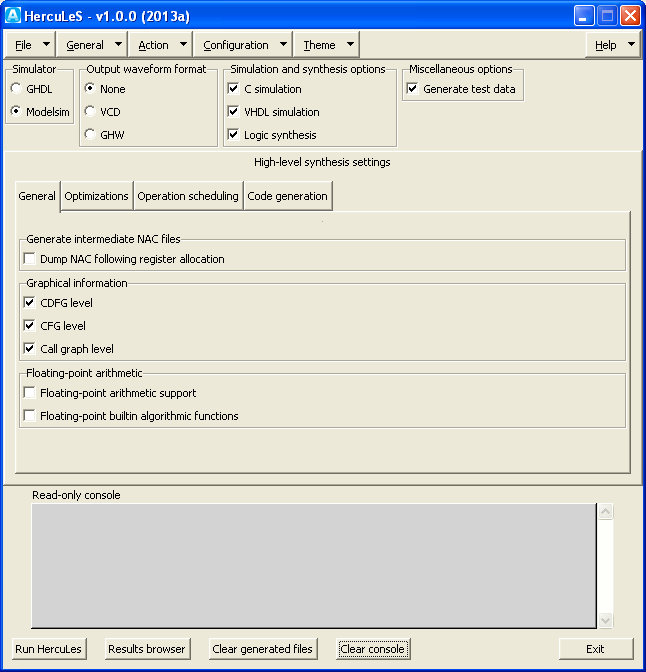
\includegraphics[scale=0.400000]{hercules-gui-basicscreen-winnative.png}}
\caption{Basic GUI screen using the \texttt{winnative} theme on Windows.}
\end{figure}


\paragraph{8.4.1.6~~~Help submenu%
  \label{help-submenu}%
}

The sixth and last dropdown menu is \texttt{Help} from which the PDF and HTML version of the HercuLeS reference manual can be accessed, by pressing the \texttt{HTML manual} and \texttt{PDF manual} menubuttons respectively. When invoked, an external HTML browser and PDF viewer (based on the default settings of the host system) will be called for viewing. When \texttt{About} is pressed the following message is generated, for version 1.0.0 (2013a) of the HercuLeS distribution.
%
\begin{quote}{\ttfamily \raggedright \noindent
HercuLeS\\
Ajax~Compilers~<info@ajaxcompilers.com>\\
Developed~by~Nikolaos~Kavvadias\\
<nkavvadias@ajaxcompilers.com>\\
Version~1.0.0~(29-Jun-2013)\}
}
\end{quote}

Fig. \hyperref[hercules-gui-ddmenu-help]{hercules-gui-ddmenu-help} illustrates the corresponding submenu.
\begin{figure}
\phantomsection\label{hercules-gui-ddmenu-help}
\noindent\makebox[\textwidth][c]{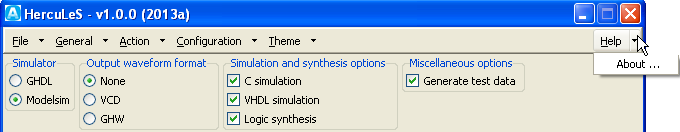
\includegraphics[scale=0.400000]{hercules-gui-ddmenu-help.png}}
\caption{Dropdown menu for accessing help and about information.}
\end{figure}


\subsubsection{8.4.2~~~Framed controls%
  \label{framed-controls}%
}

A set of basic controls are always visible as part of the basic screen layout of the HercuLeS GUI. Fig. \hyperref[hercules-gui-framedcontrols]{hercules-gui-framedcontrols} illustrates all the available basic framed controls.
\begin{figure}
\phantomsection\label{hercules-gui-framedcontrols}
\noindent\makebox[\textwidth][c]{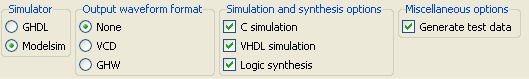
\includegraphics[scale=0.400000]{hercules-gui-framedcontrols.png}}
\caption{Controls always visible in the basic screen layout.}
\end{figure}


\paragraph{8.4.2.1~~~Simulator control%
  \label{simulator-control}%
}

The \texttt{Simulator} control provides a choice between different HDL simulators. Currently, only VHDL simulation is needed since only VHDL RTL code is generated as a result of the high-level synthesis process. The available choices for simulators are \texttt{GHDL} (for the \href{http://ghdl.free.fr}{GHDL} simulator) and \texttt{Modelsim} (for Mentor \href{http://www.model.com}{Modelsim}). It is expected that both of these simulators (or at least the one that is intended for use) is already installed on the host system and its executables directory is declared within the \texttt{PATH} environmental variable.


\paragraph{8.4.2.2~~~Output waveform format control%
  \label{output-waveform-format-control}%
}

The \texttt{Output waveform format} control allows to choose between three choices for generating or not waveform data from the HDL simulation:
%
\begin{itemize}

\item \texttt{None}: do not generate any kind of waveform data

\item \texttt{VCD}: generate waveform as Value Change Dump (VCD)

\item \texttt{GHW}: generate GHDL Waveform (GHW) data

\end{itemize}

\texttt{VCD} and \texttt{GHW} are both supported by recent versions of the \href{http://sourceforge.net/projects/gtkwave}{GTKwave} waveform viewer.


\paragraph{8.4.2.3~~~Simulation and synthesis options control%
  \label{simulation-and-synthesis-options-control}%
}

The \texttt{Simulation and synthesis options} control is a set of checkbuttons to enable or disable the generation of corresponding entries in the HercuLeS run script for the following:
%
\begin{itemize}

\item running a C simulation using the C backend files generated by a NAC-to-C decompilation process (\texttt{C simulation})

\item running an HDL simulation using either specified simulator (\texttt{VHDL simulation})

\item invoke the Xilinx ISE/XST logic synthesis tool (\texttt{Logic synthesis})

\end{itemize}


\paragraph{8.4.2.4~~~Miscellaneous options%
  \label{miscellaneous-options}%
}

The \texttt{Miscellaneous options} control groups all remaining controls. Currently only \texttt{Generate test data} is available. When enabled, this checkbutton enables using the host C compiler for generating reference test input/output data for the application under processing.


\subsubsection{8.4.3~~~Notebook controls%
  \label{notebook-controls}%
}

In order to control in detail the available high-level synthesis settings, a notebook (currently consisting of four tabs) is always accessible from the basic screen layout of the HercuLeS GUI.

These tabs organize \texttt{General}, \texttt{Optimizations}, \texttt{Operation scheduling} and \texttt{Code generation} controls into corresponding categories.


\paragraph{8.4.3.1~~~General tab%
  \label{general-tab}%
}

From left to right, the first notebook tab is \texttt{General} which covers general file emission options. It is shown in Fig. \hyperref[hercules-gui-nb-general]{hercules-gui-nb-general} and consists of three option groups.
\begin{figure}
\phantomsection\label{hercules-gui-nb-general}
\noindent\makebox[\textwidth][c]{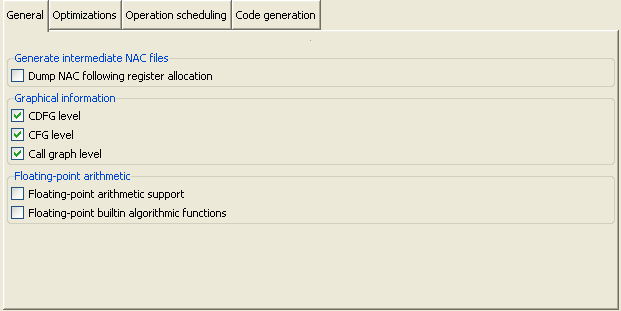
\includegraphics[scale=0.400000]{hercules-gui-nb-general.png}}
\caption{Notebook tab for general high-level synthesis settings.}
\end{figure}

The first option group, \texttt{Generate intermediate NAC files}, can be used to enable intermediate dumps after various stages of the HLS compilation process. Currently on printing intermediate NAC files for each procedure following register allocation can be specified.

The second option group, \texttt{Graphical information}, can be used for enabling and disabling of the emission of graphical information at the \texttt{CDFG} (Control-Data Flow Graph), \texttt{CFG} (Control-Flow Graph) and \texttt{Call graph} level. A CDFG illustates control and data dependencies between the statements in a NAC procedure. A CFG illustrates only the control dependencies at basic block granularity in a procedure. A call graph depicts the call graph structure of the entire translation unit.

The third option group, \texttt{Floating-point arithmetic}, provides control settings for the support of floating-point arithmetic (\texttt{Floating-point arithmetic support}). Another checkbutton, \texttt{Floating-point builtin algorithmic functions} enables the rewriting of NAC programs so that transcendental standard C library functions (such as calls to \texttt{sin()} and \texttt{atan()}) to be replaced by non-synthesizable implementations provided by proposed extensions to the VHDL-2008 floating-point arithmetic package.


\paragraph{8.4.3.2~~~Optimizations tab%
  \label{optimizations-tab}%
}

The second notebook tab is \texttt{Optimizations} which covers optimization-specific options. All depicted optimizations regard external optimizers that are bundled within the HercuLeS distributions for transforming C, NAC, or Graphviz representations. The notebook view is shown in Fig. \hyperref[hercules-gui-nb-opt]{hercules-gui-nb-opt} and consists of three option groups.
\begin{figure}
\phantomsection\label{hercules-gui-nb-opt}
\noindent\makebox[\textwidth][c]{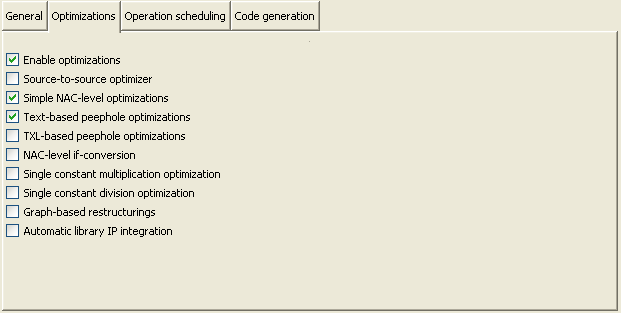
\includegraphics[scale=0.400000]{hercules-gui-nb-opt.png}}
\caption{Notebook tab for optimization settings.}
\end{figure}

This tab basically groups a set of checkbuttons for enabling or disabling specific optimizations. The first checkbutton, \texttt{Enable optimizations}, enables or disables the entire group of the following checkbuttons. The supported optimizations are as follows:
%
\begin{itemize}

\item Source-to-source optimizer:
The \texttt{txlcopt} optimizer which is a collection of C-to-C transformation passes developed in the TXL functional programming language. \texttt{txlcopt} supports arithmetic-oriented, loop-based and generic restructuring transformations.

\item Simple NAC-level optimizations:
TXL transformations written for NAC programs.

\item Text-based peephole optimizations
A collection of optimizations on NAC code applied with the help of the \texttt{copt} text-based peephole optimizer.

\item NAC-level if-conversion:
If conversion transformation applied on NAC programs. This transformation cannot be guaranteed to always produce valid code since it is purely syntax-driven and should only be used with care.

\item Single constant multiplication optimization:
Automatic replacement of single constant multiplications by optimized multiplierless routines at the NAC level.

\item Single constant division optimization:
Automatic replacement of single constant divisions by optimized divisionless routines at the NAC level.

\item Graph-based restructurings:
A set of \texttt{gvpr} transformations for use on Graphviz graphs. \texttt{gvpr} provides a scripting language interface for manipulating graphs expressed in the Graphviz language similar to \texttt{awk}.

\item Automatic library IP integration:
This option enables the automatic replacement the uses of specific VHDL operators (e.g. variable multiplications and divisions) by optimized library IP. HercuLeS takes care of all the required integration and interconnection effort associated with this task.

\end{itemize}


\paragraph{8.4.3.3~~~Operation scheduling tab%
  \label{operation-scheduling-tab}%
}

The third notebook tab is \texttt{Operation scheduling} which covers operation scheduling and memory synthesis options. Overall, this tab is dedicated for the setting of options that control aspects of the generated HDL architectures. A typical tab view is shown in Fig. \hyperref[hercules-gui-nb-arch]{hercules-gui-nb-arch} and consists of two option groups.
\begin{figure}
\phantomsection\label{hercules-gui-nb-arch}
\noindent\makebox[\textwidth][c]{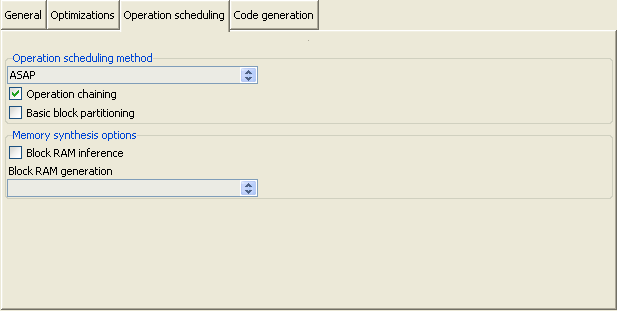
\includegraphics[scale=0.400000]{hercules-gui-nb-arch.png}}
\caption{Notebook tab for architecture-specific high-level synthesis settings.}
\end{figure}

The first option group, \texttt{Operation scheduling method}, can be used for selecting one of the provided schedulers for the task of operation scheduling. Currently \texttt{Sequential} and \texttt{ASAP} scheduling are supported. \texttt{Sequential} schedules one operation per FSMD state. \texttt{ASAP} is a form of unconstrained scheduling and allows for mutually-independent operations to be bundled within the same FSMD control step (state).

The \texttt{Operation chaining} checkbutton enables a heuristic that allows to collapse multiple dependent operations within the same FSMD control step. In some cases, this technique leads to overcontention of specific FSMD states and subsequently to lower performance (e.g. reduced clock period due to larger combinational path). \texttt{Basic block partitioning} contributes a heuristic so that existing basic blocks are split into smaller ones in order to alleviate for this problem.

The second option group is named \texttt{Memory synthesis options} and is used for controlling the generation of RAM description that support automatic block RAM inference. This mandates the use of synchronous read descriptions. Xilinx block RAM support different read schemes. The corresponding combobox, \texttt{Block RAM generation} enables the user to select among two different schemes, \texttt{Read-first} and \texttt{Read-through}. Both schemes are explained in the Xilinx \href{http://www.xilinx.com/support/documentation/application_notes/xapp463.pdf}{XAPP463} application note on block RAM usage.


\paragraph{8.4.3.4~~~Code generation tab%
  \label{code-generation-tab}%
}

The fourth and last notebook tab is \texttt{Code generation} which covers options that affect code generation in HercuLeS. A view of this tab is shown in Fig. \hyperref[hercules-gui-nb-cgen]{hercules-gui-nb-cgen} and consists of three option groups regarding backend code generation, SSA (Static Single Assignment) and register allocation.
\begin{figure}
\phantomsection\label{hercules-gui-nb-cgen}
\noindent\makebox[\textwidth][c]{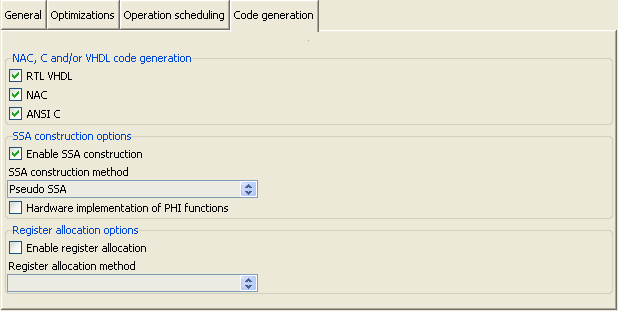
\includegraphics[scale=0.400000]{hercules-gui-nb-cgen.png}}
\caption{Notebook tab for code generation settings.}
\end{figure}

The first option group, \texttt{NAC, C and VHDL code generation}, provides checkbuttons for controlling the emission of NAC, backend ANSI C and RTL VHDL code. NAC and ANSI C backend code are generated by the \texttt{nac2cdfg} tool, while RTL VHDL is generated by the graph-based \texttt{cdfg2hdl} backend tool of HercuLeS.

This is followed by \texttt{SSA construction options}, a control set for fine-tuning the generated intermediate representation form by \texttt{nac2cdfg}. Generating SSA form is mandatory for non-sequential operation scheduling like the \texttt{ASAP} scheme. Apart from the \texttt{Enable SSA construction} checkbutton, a combobox permits to choose among two different methods for IR construction, classic minimal SSA which can be generated by using the \texttt{Aycock-Horspool} technique and \texttt{Pseudo SSA} which is a form of intrablock variable numbering. The latter is much faster than the former, however not a true SSA scheme, since the single definition point property of SSA form is not sustained at interblock scope. Another checkbutton, \texttt{Hardware implementation of PHI functions} allows for a direct mapping of \href{http://en.wikipedia.org/wiki/Static_single_assignment_form}{SSA} form (which involves so-called PHI functions which are join points for variable definitions from different control paths) to hardware. The default choice is to first convert SSA form out-of-SSA. In this case, PHI functions are removed and move operations must be placed to construct all necessary variable copies.

\texttt{Register allocation options} is a set of controls for setting whether register allocation is to be applied. When register allocation is disabled, simply its temporary variable is translated to a hardware register. To perform register allocation the \texttt{Enable register allocation} checkbutton must be selected. Currently only linear-scan register allocation (\texttt{Linear scan}) can be selected from the corresponding register allocation method combobox.


\subsubsection{8.4.4~~~Action buttons%
  \label{action-buttons}%
}

A set of five action buttons, \texttt{Run HercuLeS}, \texttt{Results browser}, \texttt{Clear generated files}, \texttt{Clear console} (on the left), and \texttt{Exit} (on the right) is visible near the bottom of the basic screen layout. Fig. \hyperref[hercules-gui-basicscreen-actions]{hercules-gui-basicscreen-actions} illustrates the corresponding controls.
\begin{figure}
\phantomsection\label{hercules-gui-basicscreen-actions}
\noindent\makebox[\textwidth][c]{
\includegraphics[scale=0.400000]{hercules-gui-basicscreen-actions.png}}
\caption{Action buttons situated near the bottom of the basic screen layout.}
\end{figure}

The actions performed by \texttt{Run HercuLeS} and \texttt{Results browser} have been already described. \texttt{Clear generated files} deletes all generated result files from the working directory of the loaded C or NAC program file. \texttt{Clear console} deletes all  information that has been emitted in the read-only console. \texttt{Exit} forces the HercuLeS GUI to close. It should be noted that \texttt{Results browser}, \texttt{Clear generated files} and \texttt{Clear console} are only enabled following the execution of a HercuLeS script.


\subsubsection{8.4.5~~~Results browser%
  \label{results-browser}%
}

The HercuLeS GUI comes with a results browser which is invoked after the execution of a HercuLeS run script has completed. Fig. \hyperref[hercules-gui-resbrowser]{hercules-gui-resbrowser} illustrates an example view of the results browser layout.
\begin{figure}
\phantomsection\label{hercules-gui-resbrowser}
\noindent\makebox[\textwidth][c]{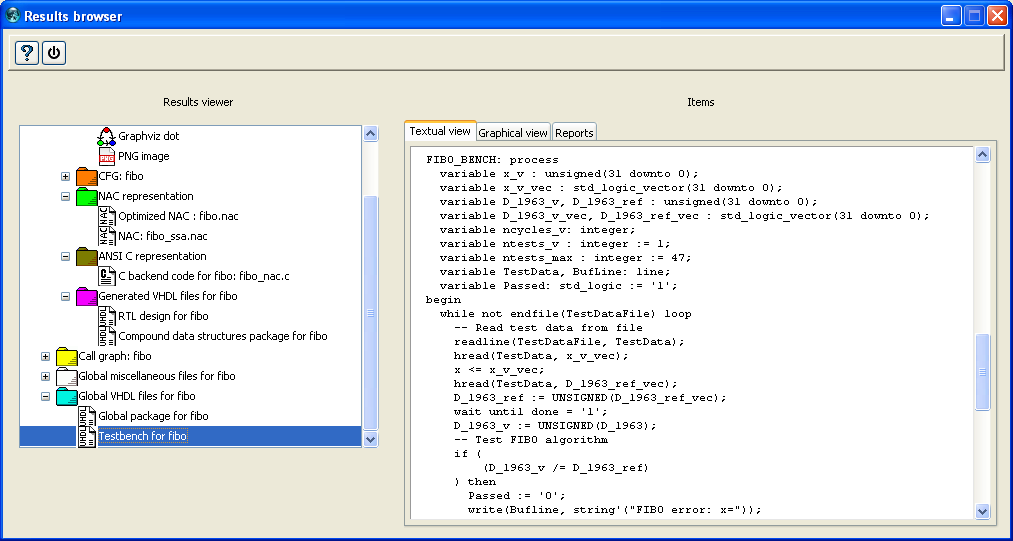
\includegraphics[scale=0.400000]{hercules-gui-resbrowser.png}}
\caption{The HercuLeS GUI results browser.}
\end{figure}

On the left side, the results browser uses a tree viewing GUI element. This tree viewer loads a file named \texttt{hlsrestree.tcl} from the application's current (working) directory. This file provides an automatically-generated GRIDPLUS tree widget to enable browsing of generated files from the high-level synthesis process.

An example \texttt{hlsrestree.tcl} automatically generated for a Fibonacci series (\texttt{fibo}) computation application is shown below:
%
\begin{quote}{\ttfamily \footnotesize \raggedright \noindent
gpset~.treebrowser.hlstree~\{\\
~~\{/PRGM~+~"Program:~fibo"~:folder\_blue-22\}\\
~~\{/PRGM/RPTS~+~"Reports"~:folder\_graph\_white-22\}\\
~~\{/PRGM/RPTS/RESANSIC~"ANSI~C~simulation~results"~:txt-22\}\\
~~\{/PRGM/RPTS/RESVHDL~"VHDL~simulation~results"~:txt-22\}\\
~~\{/PRGM/RPTS/RESXST~"XST/ISE~synthesis~report"~:txt-22\}\\
~~\{/PRGM/PROC0~+~"Procedure:~fibo"~:folder\_grey-22\}\\
~~\{/PRGM/PROC0/CDFG~+~"CDFG:~fibo"~:folder\_red-22\}\\
~~\{/PRGM/PROC0/CDFG/DOT~"Graphviz~dot"~:dot-22\}\\
~~\{/PRGM/PROC0/CDFG/PNG~"PNG~image"~:png-22\}\\
~~\{/PRGM/PROC0/CFG~+~"CFG:~fibo"~:folder\_orange-22\}\\
~~\{/PRGM/PROC0/CFG/DOT~"Graphviz~dot"~:dot-22\}\\
~~\{/PRGM/PROC0/CFG/PNG~"PNG~image"~:png-22\}\\
~~\{/PRGM/PROC0/NAC~+~"NAC~representation"~:folder\_green-22\}\\
~~\{/PRGM/PROC0/NAC/FINAL~"Optimized~NAC~:~fibo.nac"~:nac-22\}\\
~~\{/PRGM/PROC0/NAC/POSTFE~"NAC:~fibo\_ssa.nac"~:nac-22\}\\
~~\{/PRGM/PROC0/ANSIC~+~"ANSI~C~representation"~:folder\_olive-22\}\\
~~\{/PRGM/PROC0/ANSIC/FINAL~"C~backend~code~for~fibo:~fibo\_nac.c"~:ansic-22\}\\
~~\{/PRGM/PROC0/VHDL~+~"Generated~VHDL~files~for~fibo"~:folder\_magenta-22\}\\
~~\{/PRGM/PROC0/VHDL/RTL~"RTL~design~for~fibo"~:vhdl-22\}\\
~~\{/PRGM/PROC0/VHDL/CDTPKG~"Compound~data~structures~package~for~fibo"~:vhdl-22\}\\
~~\{/PRGM/CG~+~"Call~graph:~fibo"~:folder\_yellow-22\}\\
~~\{/PRGM/CG/DOT~"Graphviz~dot"~:dot-22\}\\
~~\{/PRGM/CG/PNG~"PNG~image"~:png-22\}\\
~~\{/PRGM/GLOBAL~+~"Global~miscellaneous~files~for~fibo"~:folder\_white-22\}\\
~~\{/PRGM/GLOBAL/HERCSH~"Generated~HercuLeS~bash~script~for~fibo"~:bash-22\}\\
~~\{/PRGM/GLOBAL/PROCNMS~"Procedure~names~in~fibo"~:txt-22\}\\
~~\{/PRGM/GLOBAL/BUILTINS~"Black~box~procedures~in~fibo"~:txt-22\}\\
~~\{/PRGM/GLOBAL/TESTDATA~"Reference~I/O~data~for~fibo"~:txt-22\}\\
~~\{/PRGM/GLOBAL/MAINC~"C~driver~code~for~fibo:~main.c"~:ansic-22\}\\
~~\{/PRGM/GLOBAL/MAINH~"C~header~code~for~fibo:~main.h"~:ansic\_header-22\}\\
~~\{/PRGM/GLOBAL/MK~"Makefile~for~builting~C~backend~code:~ansic.mk"~:makefile-22\}\\
~~\{/PRGM/GLOBAL/RSIMDO~".do~script~for~VHDL~simulation~using~Modelsim"~:txt-22\}\\
~~\{/PRGM/GLOBAL/RSIMSH~"Bash~script~for~running~the~VHDL~simulation"~:bash-22\}\\
~~\{/PRGM/GLOBAL/XSTSH~"Bash~script~for~running~logic~synthesis~with~Xilinx~XST/ISE"~:bash-22\}\\
~~\{/PRGM/VHDL~+~"Global~VHDL~files~for~fibo"~:folder\_cyan-22\}\\
~~\{/PRGM/VHDL/PKG~"Global~package~for~fibo"~:vhdl-22\}\\
~~\{/PRGM/VHDL/TB~"Testbench~for~fibo"~:vhdl-22\}\\
\}
}
\end{quote}

On the right side, the user can view either a textual or a graphical representation (the latter when appropriate) of the requested information. Currently, the \texttt{Graphical view} and \texttt{Statistics} views are left unused. It should be noted that when requesting a PNG visualization of a graph (e.g. a CDFG, CFG or call graph), an external image viewer is accessed, the name of and the path to which can be defined via means of the initialization file or the external tools configuration layout.

The following table summarizes all automatically generated files that are accessible from the results browser environment. The name of the current application is \texttt{app}.

{\footnotesize 
\setlength{\DUtablewidth}{\linewidth}
\begin{longtable*}[c]{|p{0.319\DUtablewidth}|p{0.610\DUtablewidth}|}
\hline

Path to tree widget
 & 
Description
 \\
\hline

/PRGM
 & 
Top-level folder for \texttt{app}.
 \\
\hline

/PRGM/REPORTS
 & 
Reports folder.
 \\
\hline

/PRGM/REPORTS/DEBUG

/PRGM/REPORTS/RESANSIC

/PRGM/REPORTS/RESVHDL

/PRGM/REPORTS/RESXST
 & 
Debug dump.

ANSI C simulation results.

VHDL simulation results.

XST/ISE synthesis report.
 \\
\hline

/PRGM/PROC\$i
 & 
Top-level folder for procedure \texttt{proc}.
 \\
\hline

/PRGM/PROC\$i/CDFG
 & 
CDFG folder for \texttt{proc}.
 \\
\hline

/PRGM/PROC\$i/CDFG/DOT

/PRGM/PROC\$i/CDFG/PNG
 & 
Graphviz dot representation for the CDFG.

PNG image visualization of the Graphviz CDFG.
 \\
\hline

/PRGM/PROC\$i/CFG
 & 
CFG folder for \texttt{proc}.
 \\
\hline

/PRGM/PROC\$i/CFG/DOT

/PRGM/PROC\$i/CFG/PNG
 & 
Graphviz dot representation for the CFG.

PNG image visualization for the CFG.
 \\
\hline

/PRGM/PROC\$i/NAC
 & 
Folder for the NAC representation of \texttt{proc}.
 \\
\hline

/PRGM/PROC\$i/NAC/FINAL

/PRGM/PROC\$i/NAC/POSTFE

/PRGM/PROC\$i/NAC/RA
 & 
Optimized NAC for \texttt{proc}.

NAC following frontend processing for \texttt{proc}.

NAC following register allocation for \texttt{proc}.
 \\
\hline

/PRGM/PROC\$i/ANSIC
 & 
Folder for the ANSI C representation of \texttt{proc}.
 \\
\hline

/PRGM/PROC\$i/ANSIC/FINAL
 & 
C backend code for \texttt{proc}.
 \\
\hline

/PRGM/PROC\$i/VHDL
 & 
Folder for generated VHDL files of \texttt{proc}.
 \\
\hline

/PRGM/PROC\$i/VHDL/RTL

/PRGM/PROC\$i/VHDL/CDTPKG
 & 
RTL design for \texttt{proc}.

Compound data structures package for \texttt{proc}.
 \\
\hline

/PRGM/CG
 & 
Call graph for \texttt{app}.
 \\
\hline

/PRGM/CG/DOT

/PRGM/CG/PNG
 & 
Graphviz dot representation for the call graph.

PNG image visualization for the call graph.
 \\
\hline

/PRGM/GLOBAL
 & 
Global miscellaneous files for \texttt{app}.
 \\
\hline

/PRGM/GLOBAL/HERCSH

/PRGM/GLOBAL/PROCNMS

/PRGM/GLOBAL/BUILTINS

/PRGM/GLOBAL/TESTDATA

/PRGM/GLOBAL/MAINC

/PRGM/GLOBAL/MAINH

/PRGM/GLOBAL/MK

/PRGM/GLOBAL/RSIMMK

/PRGM/GLOBAL/RSIMDO

/PRGM/GLOBAL/RSIMSH

/PRGM/GLOBAL/XSTSH
 & 
Generated HercuLeS bash script for \texttt{app}.

Procedure names in \texttt{app}.

Black box procedures in \texttt{app}.

Reference I/O data for \texttt{app}.

C driver code for \texttt{app}.

C header code for \texttt{app}.

Makefile for builting C backend code.

Makefile for VHDL simulation using GHDL.

\texttt{.do} script for VHDL simulation using Modelsim.

Bash script for running the VHDL simulation.

Bash script for running logic synthesis.
 \\
\hline

/PRGM/VHDL
 & 
Folder for global VHDL files of \texttt{app}.
 \\
\hline

/PRGM/VHDL/PKG

/PRGM/VHDL/TB
 & 
Global package for \texttt{app}.

Testbench for \texttt{app}.
 \\
\hline
\end{longtable*}
}

\subsection{8.5~~~Configuration files%
  \label{configuration-files}%
}

HercuLeS supports user-defined configuration files for fast loading of high-level synthesis settings. A configuration file is expected to have the \texttt{.config} suffix. The supplied options are organized into four distinct categories, \texttt{common} (options that are common across all tools), \texttt{nac2cdfg} (passed to the HercuLeS \texttt{nac2cdfg} tool), \texttt{cdfg2hdl} (passed to the HercuLeS \texttt{cdfg2hdl} tool) and \texttt{more} where all miscellaneous options are defined. For the first three categories, these options represent command-line switches. The last category, \texttt{more}, defines options that are intentionally similar to command-line switches but are however passed to the HercuLeS GUI directly for controlling HercuLeS run script generation.

The general structure of a configuration file is shown below:
%
\begin{quote}{\ttfamily \raggedright \noindent
start-common\\
<options>\\
end-common\\
~\\
start-nac2cdfg\\
<options>\\
end-nac2cdfg\\
~\\
start-cdfg2hdl\\
<options>\\
end-cdfg2hdl\\
~\\
start-more\\
<options>\\
end-more
}
\end{quote}

An example of a typical configuration file invoking C backend file simulation, VHDL simulation and XST/ISE synthesis is shown below:
%
\begin{quote}{\ttfamily \raggedright \noindent
start-common\\
end-common\\
~\\
start-nac2cdfg\\
-force-data-types\\
-ssa\\
-pseudo-ssa\\
-emit-nac\\
-emit-ansic\\
-emit-cfg\\
-emit-cg\\
end-nac2cdfg\\
~\\
start-cdfg2hdl\\
-sched-asap\\
-ieee\\
-vhd2vl\\
-mpint\\
-mti\\
end-cdfg2hdl\\
~\\
start-more\\
-optimizations\\
-nacsopt\\
-nacpeep\\
-chain\\
-rsim\\
-csim\\
-datagen\\
-synth\\
-emit-cdfg\\
end-more
}
\end{quote}

The list of command-line switches that are passed to the HercuLeS GUI is as follows:
%
\begin{description}
\item[{-optimizations:}] \leavevmode 
Enable optimizations.

\item[{-srcopt:}] \leavevmode 
Source-to-source optimizer.

\item[{-nacsopt:}] \leavevmode 
Simple NAC-level optimizations.

\item[{-nacpeep:}] \leavevmode 
Text-based peephole optimizations.

\item[{-txlpeep:}] \leavevmode 
TXL-based peephole optimizations.

\item[{-nacifconv:}] \leavevmode 
NAC-level if-conversion.

\item[{-kmul:}] \leavevmode 
Single constant multiplication optimization.

\item[{-kdiv:}] \leavevmode 
Single constant division optimization.

\item[{-gvpropt:}] \leavevmode 
Graph-based restructurings applied on Graphviz CDFG graphs.

\item[{-ipopt:}] \leavevmode 
Automatic library IP integration.

\item[{-bbpart:}] \leavevmode 
Enable basic block partitioning.

\item[{-emit-vhdl:}] \leavevmode 
Emit RTL VHDL code.

\item[{-xst-script:}] \leavevmode 
Generate a script for driving Xilinx XST/ISE logic synthesis.

\item[{-rsim:}] \leavevmode 
Enable VHDL simulation.

\item[{-csim:}] \leavevmode 
Enable backend C code simulation.

\item[{-datagen:}] \leavevmode 
Generate reference input/output data for the loaded application.

\item[{-emit-cdfg:}] \leavevmode 
Generate Graphviz CDFGs and their PNG visualizations for the application.

\item[{-synth:}] \leavevmode 
Enable logic synthesis.

\end{description}


\subsection{8.6~~~Initialization file%
  \label{initialization-file}%
}

During startup, the HercuLeS GUI automatically loads a predefined initialization file, named \texttt{hercules.ini}. This \texttt{.ini} file assigns all required environmental and internal variables for the proper setup of HercuLeS.

The initialization file is an ASCII text file comprising of a set of entries of the following form:

\begin{DUlineblock}{0em}
\item[] \texttt{variable="rhs-string"}
\end{DUlineblock}

where \texttt{variable} is the name of the environmental or internal use variable to be set and \texttt{rhs-string} is the string value that is assigned to it.

The following table provides a brief summary of the variables that can be defined in initialization files.

\setlength{\DUtablewidth}{\linewidth}
\begin{longtable*}[c]{|p{0.261\DUtablewidth}|p{0.668\DUtablewidth}|}
\hline

Name
 & 
Description
 \\
\hline

hlstop
 & 
Top-level installation directory for HercuLeS.
 \\
\hline

compiler\_name
 & 
Name of the host C compiler.
 \\
\hline

compiler\_path
 & 
Path to the executables' directory of the host C
compiler.
 \\
\hline

compiler\_opts
 & 
Command-line options to pass to the host C compiler for
generating GIMPLE dumps (only for \texttt{gcc} and
\texttt{gimple2nac}).
 \\
\hline

cfe\_name
 & 
Name of the C frontend for compiling to NAC.
 \\
\hline

cfe\_path
 & 
Path to the C frontend executable.
 \\
\hline

srcopt\_path
 & 
Path to the C-to-C optimizer.
 \\
\hline

xilinx\_ise\_path
 & 
Path to the Xilinx ISE directory.
 \\
\hline

fpga\_arch
 & 
FPGA architecture to be used for logic synthesis.
 \\
\hline

fpga\_part
 & 
FPGA device to be used for logic synthesis.
 \\
\hline

graphviz\_path
 & 
Path to the Graphviz installation.
 \\
\hline

dotproc\_name
 & 
Name of the Graphviz dot processor (default: \texttt{dot}).
 \\
\hline

dotviewer\_name
 & 
Name of the Graphviz file viewer (default: \texttt{dotty}).
 \\
\hline

imgviewer\_name
 & 
Name of the image viewer executable.
 \\
\hline

imgviewer\_path
 & 
Path to the image viewer executables' directory.
 \\
\hline

pdfviewer\_name
 & 
Name of the PDF viewer executable.
 \\
\hline

pdfviewer\_path
 & 
Path to the PDF viewer executables' directory.
 \\
\hline

htmlviewer\_name
 & 
Name of the HTML viewer executable.
 \\
\hline

htmlviewer\_path
 & 
Path to the HTML viewer executables' directory.
 \\
\hline
\end{longtable*}

An example initialization file is shown below:
%
\begin{quote}{\ttfamily \raggedright \noindent
hlstop="g:/hercules"\\
compiler\_name="gcc"\\
compiler\_path="/usr/local/bin/gcc-4.7.0-install/bin"\\
compiler\_opts="-Wall~-O2~-fdump-tree-gimple-raw"\\
cfe\_name="gimple2nac"\\
cfe\_path="g:/hercules/gimple2nac"\\
srcopt\_path="g:/hercules/txlcopt"\\
xilinx\_ise\_path="c:/Xilinx/12.3/ISE\_DS/ISE"\\
fpga\_arch="virtex6"\\
fpga\_part="xc6vlx75t-ff484-1"\\
graphviz\_path="c:/CompSci/Graphviz2.28"\\
imgviewer\_path="g:/hercules/thirdparty/Imagine"\\
imgviewer\_name="Imagine"\\
dotproc\_name="dot"\\
dotviewer\_name="dotty"\\
pdfviewer\_path="c:/Program\textbackslash{}~Files/Adobe/Reader\textbackslash{}~10.0/Reader"\\
pdfviewer\_name="AcroRd32"\\
htmlviewer\_path="c:/Documents\textbackslash{}~and\textbackslash{}~Settings/nkavvadias/Local\textbackslash{}~Settings/Application\textbackslash{}~Data/Google/Chrome/Application"\\
htmlviewer\_name="chrome"
}
\end{quote}

% Local Variables:
% mode: indented-text
% indent-tabs-mode: nil
% sentence-end-double-space: t
% fill-column: 72
% End:

\end{document}
